

%\todo[inline]{I (Ludovic) can make the blabla about the tree theorem with references in literature to motivate this section, unless Benoit, you feel like to make it.}

In this chapter, we study the principle $\mathrm{CHMTT^n_{k,l}}$ stating that given a $k$-coloring of $[2^{<\omega}]^n$, there is a subtree $S\subseteq 2^{<\omega}$ such that $(S, \preceq)$ is isomorphic to $(2^{<\omega}, \preceq)$ and such that $[S]^n$ uses at most $l$ colors. Note that we do not require $S$ to be a strong subtree of $T$ or even $S$ to be meet-closed --- thus enlarging a bit for this chapter the original definition of a tree given with \cref{def:trees}. 

The existence for every $n$ of a finite big Ramsey degree associated with these structures --- a smallest number $l_n$ such that $\mathrm{CHMTT^n_{k,l_n}}$ holds for every $k$ --- easily follows from the Milliken's tree theorem. We will try to identify more precisely the specific values of these big Ramsey degrees $l_n$, a new sequence of numbers, which does not seem to have appeared before in combinatorics.

In order to pursue this study, we introduce first a simpler principle, for which we now require the subtree to be a strong subtree.

\begin{theorem}[Strong generalized CHM tree theorem]\index{generalized CHM tree theorem!strong}\index{tree theorem!strong generalized CHM tree theorem}
For every $n \geq 1$ there exists $\ell \geq 1$ such that for every $k \geq 1$ and every $f: [2^{<\omega}]^n \to k$ there is a strong subtree $S \subseteq 2^{<\omega}$ such that $|f ([S]^n)| \leq \ell$. 
\end{theorem}
\begin{statement}\index{statement!$\mathrm{SCHMTT^n_{k,l}}$}
  We call $\mathrm{SCHMTT^n_{k,l}}$ the statement of the Strong generalized CHM tree theorem.
\end{statement}

Note that both $\mathrm{SCHMTT^n_{k,l}}$ and $\mathrm{CHMTT^n_{k,l}}$ would work exactly the same way if we start from a coloring of any perfect tree $T$ rather than $2^{<\omega}$: via an isomorphism between $T$ and $2^{<\omega}$, the theorem applied to $2^{<\omega}$ also gives via the isomorphism a solution for $T$. We start by introducing the notion of embedding types, useful in the conduct of our study.

\section{Embedding types}

We shall try to identify what can be used by a coloring of $[2^{<\omega}]^n$ to identify some structure one will never be able to remove in any strong subtree. A first step for that is the identification of the concept of embedding type, for which we introduce the following preliminary notions.

\begin{definition}
Let $S$ be a set of strings.
\begin{enumerate}\index{meet-closed}\index{level-closed}
\item $S$ is \emph{meet-closed} if for every $\sigma,\tau\in S$, $\sigma \wedge \tau \in S$. 
\item $S$ is \emph{level-closed} if for every $\sigma,\tau\in S$, $\tau\uh|\sigma|\in S$.
\end{enumerate}
\end{definition}

We will be interested in finite trees which are both meet-closed and level closed. 

\begin{definition}[closure]
Let $S$ be a set of strings.
\begin{enumerate}\index{meet closure}\index{level closure}\index{full closure}\index{closure!meet}\index{closure!full}\index{closure!level}\index{$A^\wedge$}\index{$\lvlclosure A$}\index{$A^{\mathrm{cl}}$}
\item The \emph{meet closure} of $S$ is the set $S^\wedge=\{\sigma \wedge \tau:\sigma,\tau\in S\}$.
\item The \emph{level closure} of $S$ is the set $\lvlclosure S=\{\sigma\uh|\tau|:\sigma,\tau\in S\}$.
\item The \emph{full closure} of $S$ is the set $S^{\mathrm{cl}} = \lvlclosure {(S^\wedge)}$.
\end{enumerate}
\end{definition}

Note that $S \subseteq S^\wedge$ and $S \subseteq \lvlclosure S$ by taking $\sigma=\tau$ in the above definitions. Any strong subtree of $2^{<\omega}$ is meet-closed and level-closed but not conversely, as witnessed by the following example $S=\{\emptystr;0;00;01;1;11\}$. In Figure~\ref{fig:some-trees}, we give an example of a subtree, and its full closure.
\begin{figure}[h]
  \centering
  %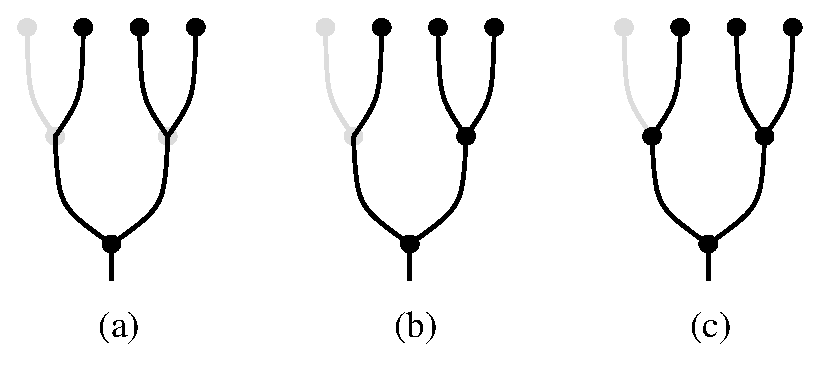
\includegraphics[scale=0.4]{figures/someTrees.eps}
  \centering
	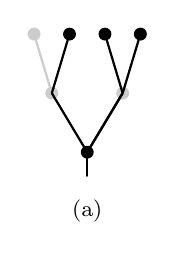
\begin{tikzpicture}[scale=1.5,font=\footnotesize]
		\tikzset{
			empty node/.style={circle,inner sep=0,fill=none},
			solid node/.style={circle,draw,inner sep=1.5,fill=black},
			hollow node/.style={circle,draw,inner sep=1.5,fill=white},
			gray node/.style={circle,draw={rgb:black,1;white,4},inner sep=1.5,fill={rgb:black,1;white,4}}
		}
		\tikzset{snake it/.style={decorate, decoration=snake, line cap=round}}
		\tikzset{gray line/.style={line cap=round,thick,color={rgb:black,1;white,4}}}
		\tikzset{thick line/.style={line cap=round,rounded corners=0.1mm,thick}}
		\node (a)[solid node] at (0,0) {};
		\node (a1)[gray node] at (0.3,0.5) {};
		\node (a0)[gray node] at (-0.3,0.5) {};
		\node (a00)[gray node] at (-0.45,1) {};
		\node (a01)[solid node] at (-0.15,1) {};
		\node (a10)[solid node] at (0.15,1) {};
		\node (a11)[solid node] at (0.45,1) {};
		\draw[-,thick line] (a) to (-0.3,0.5) to (a01);
		\draw[-,thick line] (a) to (0.3,0.5) to (a10);
		\draw[-,thick line] (a) to (0.3,0.5) to (a11);
		\draw[-,gray line] (a0) to (a00);
		\draw[-,thick line] (0,-0.2) to (a);
		\node at (0,-0.5) {(a)};
	\end{tikzpicture}
	\hspace{5mm}
	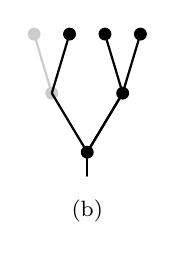
\begin{tikzpicture}[scale=1.5,font=\footnotesize]
		\tikzset{
			empty node/.style={circle,inner sep=0,fill=none},
			solid node/.style={circle,draw,inner sep=1.5,fill=black},
			hollow node/.style={circle,draw,inner sep=1.5,fill=white},
			gray node/.style={circle,draw={rgb:black,1;white,4},inner sep=1.5,fill={rgb:black,1;white,4}}
		}
		\tikzset{snake it/.style={decorate, decoration=snake, line cap=round}}
		\tikzset{gray line/.style={line cap=round,thick,color={rgb:black,1;white,4}}}
		\tikzset{thick line/.style={line cap=round,rounded corners=0.1mm,thick}}
		\node (a)[solid node] at (0,0) {};
		\node (a1)[solid node] at (0.3,0.5) {};
		\node (a0)[gray node] at (-0.3,0.5) {};
		\node (a00)[gray node] at (-0.45,1) {};
		\node (a01)[solid node] at (-0.15,1) {};
		\node (a10)[solid node] at (0.15,1) {};
		\node (a11)[solid node] at (0.45,1) {};
		\draw[-,thick line] (a) to (-0.3,0.5) to (a01);
		\draw[-,thick line] (a) to (0.3,0.5) to (a10);
		\draw[-,thick line] (a) to (0.3,0.5) to (a11);
		\draw[-,gray line] (a0) to (a00);
		\draw[-,thick line] (0,-0.2) to (a);
		\node at (0,-0.5) {(b)};
	\end{tikzpicture}
	\hspace{5mm}
	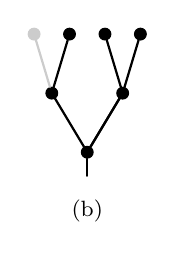
\begin{tikzpicture}[scale=1.5,font=\footnotesize]
		\tikzset{
			empty node/.style={circle,inner sep=0,fill=none},
			solid node/.style={circle,draw,inner sep=1.5,fill=black},
			hollow node/.style={circle,draw,inner sep=1.5,fill=white},
			gray node/.style={circle,draw={rgb:black,1;white,4},inner sep=1.5,fill={rgb:black,1;white,4}}
		}
		\tikzset{snake it/.style={decorate, decoration=snake, line cap=round}}
		\tikzset{gray line/.style={line cap=round,thick,color={rgb:black,1;white,4}}}
		\tikzset{thick line/.style={line cap=round,rounded corners=0.1mm,thick}}
		\node (a)[solid node] at (0,0) {};
		\node (a1)[solid node] at (0.3,0.5) {};
		\node (a0)[solid node] at (-0.3,0.5) {};
		\node (a00)[gray node] at (-0.45,1) {};
		\node (a01)[solid node] at (-0.15,1) {};
		\node (a10)[solid node] at (0.15,1) {};
		\node (a11)[solid node] at (0.45,1) {};
		\draw[-,thick line] (a) to (-0.3,0.5) to (a01);
		\draw[-,thick line] (a) to (0.3,0.5) to (a10);
		\draw[-,thick line] (a) to (0.3,0.5) to (a11);
		\draw[-,gray line] (a0) to (a00);
		\draw[-,thick line] (0,-0.2) to (a);
		\node at (0,-0.5) {(b)};
	\end{tikzpicture}
  \caption{The set of nodes (a) is level-closed but not meet-closed. The set of nodes (b) is the meet-closure of (a). Note that it is now not level-closed. The set of nodes (c) is the level-closure of (b) which corresponds to the full closure of (a).}
  \label{fig:some-trees}
\end{figure}


%\begin{lemma}The following holds:
%  \begin{enumerate}
%%  \item If $T$ is a tree and $S$ is a subtree of $T$, then $S^\meet$ is a $\meet$-closed subtree of $T$, and $\lvlclosure{S}$ is a level-closed subtree of $T$.
%  \item If $T$ is a tree and $S$ is a subtree of $T$, then $\lvlclosure{S}$ is a level-closed subtree of $T$.
%%  \item For every tree $T$ and subtree $S$ of $T$, $S\subseteq S^\meet\subseteq T$ and $S\subseteq \lvlclosure S\subseteq T$.
%  \item For every tree $T$ and subtree $S$ of $T$, $S\subseteq \lvlclosure S\subseteq T$.
%  \end{enumerate}
%\end{lemma}
  
The idea is the following: given a set of strings $S = \{\sigma_1, \dots, \sigma_n\} \in [2^{<\omega}]^n$, one can easily compute the tree $S^{\mathrm{cl}}$. A coloring can then identify which \emph{type} of tree arise from $S$ and give a different color to each of them. The number of these type is defined below as the \emph{embedding types} that we now formally define.
  
\begin{definition}\index{tree!strong isomorphism}\index{isomorphism!fully closed tree}\index{embedding type}\index{type!embedding}
Two finite fully closed trees $F_0,F_1 \subseteq 2^{<\omega}$ are \emph{strongly isomorphic} if there is a bijection $f:F_0 \rightarrow F_1$ such that $\sigma i \preceq \tau \leftrightarrow f(\sigma) i \preceq f(\tau)$ for any $\sigma, \tau \in F_0$. The \emph{embedding types} are the equivalence classes of the strong isomorphism relation on finite fully closed trees.
\end{definition}  
 
Any embedding type has a minimal element with respect its height. We usually use this minimal element as a canonical representative of the class.

\Cref{fig:same-emb-types,fig:some-emb-height,fig:some-emb-types} illustrate the notion of embedding types. \Cref{fig:some-emb-types} consists of example of different embedding types. \Cref{fig:same-emb-types} shows several level-closed subtrees with the same embedding type. \Cref{fig:some-emb-height} illustrates the height of an embedding type.

\begin{figure}[h]
%  \centering 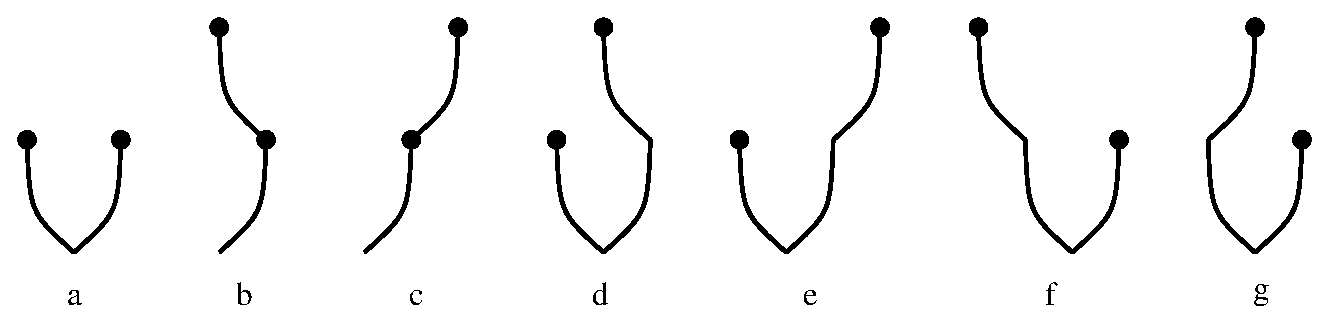
\includegraphics[scale=0.5]{embTypeExamples.eps}
  \centering
  %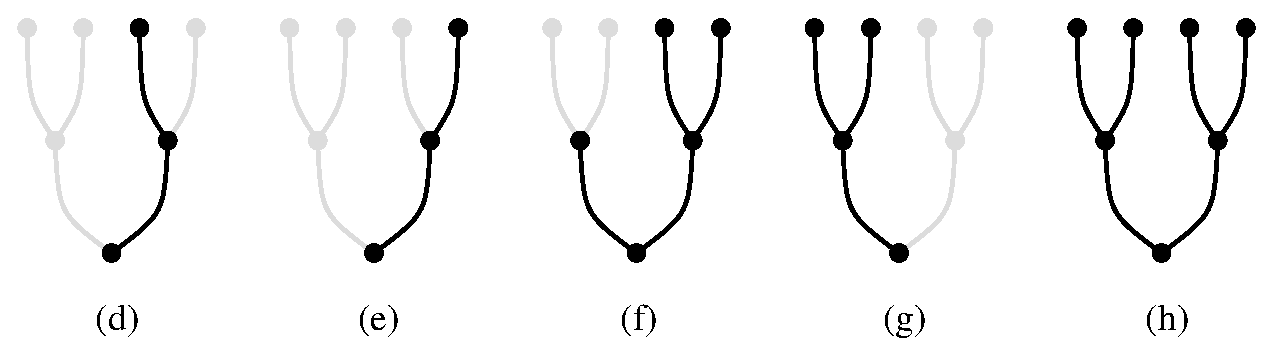
\includegraphics[scale=0.4]{figures/someEmbeddingTypes.eps}
  \begin{tikzpicture}[scale=1.5,font=\footnotesize]
		\tikzset{
			empty node/.style={circle,inner sep=0,fill=none},
			solid node/.style={circle,draw,inner sep=1.5,fill=black},
			hollow node/.style={circle,draw,inner sep=1.5,fill=white},
			gray node/.style={circle,draw={rgb:black,1;white,4},inner sep=1.5,fill={rgb:black,1;white,4}}
		}
		\tikzset{snake it/.style={decorate, decoration=snake, line cap=round}}
		\tikzset{gray line/.style={line cap=round,thick,color={rgb:black,1;white,4}}}
		\tikzset{thick line/.style={line cap=round,rounded corners=0.1mm,thick}}
		\node (a)[solid node] at (0,0) {};
		\node (a1)[solid node] at (0.3,0.5) {};
		\node (a0)[gray node] at (-0.3,0.5) {};
		\node (a00)[gray node] at (-0.45,1) {};
		\node (a01)[gray node] at (-0.15,1) {};
		\node (a10)[solid node] at (0.15,1) {};
		\node (a11)[gray node] at (0.45,1) {};
		\begin{pgfonlayer}{background}
		\draw[-,gray line] (a) to (a0);
		\draw[-,thick line] (a) to (a1);
		\draw[-,gray line] (a0) to (a00);
		\draw[-,gray line] (a0) to (a01);
		\draw[-,thick line] (a1) to (a10);
		\draw[-,gray line] (a1) to (a11);
		\end{pgfonlayer}
		\node at (0,-0.5) {(d)};
	\end{tikzpicture}
	\hspace{5mm}
	\begin{tikzpicture}[scale=1.5,font=\footnotesize]
		\tikzset{
			empty node/.style={circle,inner sep=0,fill=none},
			solid node/.style={circle,draw,inner sep=1.5,fill=black},
			hollow node/.style={circle,draw,inner sep=1.5,fill=white},
			gray node/.style={circle,draw={rgb:black,1;white,4},inner sep=1.5,fill={rgb:black,1;white,4}}
		}
		\tikzset{snake it/.style={decorate, decoration=snake, line cap=round}}
		\tikzset{gray line/.style={line cap=round,thick,color={rgb:black,1;white,4}}}
		\tikzset{thick line/.style={line cap=round,rounded corners=0.1mm,thick}}
		\node (a)[solid node] at (0,0) {};
		\node (a1)[solid node] at (0.3,0.5) {};
		\node (a0)[gray node] at (-0.3,0.5) {};
		\node (a00)[gray node] at (-0.45,1) {};
		\node (a01)[gray node] at (-0.15,1) {};
		\node (a10)[gray node] at (0.15,1) {};
		\node (a11)[solid node] at (0.45,1) {};
		\begin{pgfonlayer}{background}
		\draw[-,gray line] (a) to (a0);
		\draw[-,thick line] (a) to (a1);
		\draw[-,gray line] (a0) to (a00);
		\draw[-,gray line] (a0) to (a01);
		\draw[-,gray line] (a1) to (a10);
		\draw[-,thick line] (a1) to (a11);
		\end{pgfonlayer}
		\node at (0,-0.5) {(e)};
	\end{tikzpicture}
	\hspace{5mm}
	\begin{tikzpicture}[scale=1.5,font=\footnotesize]
		\tikzset{
			empty node/.style={circle,inner sep=0,fill=none},
			solid node/.style={circle,draw,inner sep=1.5,fill=black},
			hollow node/.style={circle,draw,inner sep=1.5,fill=white},
			gray node/.style={circle,draw={rgb:black,1;white,4},inner sep=1.5,fill={rgb:black,1;white,4}}
		}
		\tikzset{snake it/.style={decorate, decoration=snake, line cap=round}}
		\tikzset{gray line/.style={line cap=round,thick,color={rgb:black,1;white,4}}}
		\tikzset{thick line/.style={line cap=round,rounded corners=0.1mm,thick}}
		\node (a)[solid node] at (0,0) {};
		\node (a1)[solid node] at (0.3,0.5) {};
		\node (a0)[solid node] at (-0.3,0.5) {};
		\node (a00)[gray node] at (-0.45,1) {};
		\node (a01)[gray node] at (-0.15,1) {};
		\node (a10)[solid node] at (0.15,1) {};
		\node (a11)[solid node] at (0.45,1) {};
		\begin{pgfonlayer}{background}
		\draw[-,thick line] (a) to (a0);
		\draw[-,thick line] (a) to (a1);
		\draw[-,gray line] (a0) to (a00);
		\draw[-,gray line] (a0) to (a01);
		\draw[-,thick line] (a1) to (a10);
		\draw[-,thick line] (a1) to (a11);
		\end{pgfonlayer}
		\node at (0,-0.5) {(f)};
	\end{tikzpicture}
	\hspace{5mm}
	\begin{tikzpicture}[scale=1.5,font=\footnotesize]
		\tikzset{
			empty node/.style={circle,inner sep=0,fill=none},
			solid node/.style={circle,draw,inner sep=1.5,fill=black},
			hollow node/.style={circle,draw,inner sep=1.5,fill=white},
			gray node/.style={circle,draw={rgb:black,1;white,4},inner sep=1.5,fill={rgb:black,1;white,4}}
		}
		\tikzset{snake it/.style={decorate, decoration=snake, line cap=round}}
		\tikzset{gray line/.style={line cap=round,thick,color={rgb:black,1;white,4}}}
		\tikzset{thick line/.style={line cap=round,rounded corners=0.1mm,thick}}
		\node (a)[solid node] at (0,0) {};
		\node (a1)[gray node] at (0.3,0.5) {};
		\node (a0)[solid node] at (-0.3,0.5) {};
		\node (a00)[solid node] at (-0.45,1) {};
		\node (a01)[solid node] at (-0.15,1) {};
		\node (a10)[gray node] at (0.15,1) {};
		\node (a11)[gray node] at (0.45,1) {};
		\begin{pgfonlayer}{background}
		\draw[-,thick line] (a) to (a0);
		\draw[-,gray line] (a) to (a1);
		\draw[-,thick line] (a0) to (a00);
		\draw[-,thick line] (a0) to (a01);
		\draw[-,gray line] (a1) to (a10);
		\draw[-,gray line] (a1) to (a11);
		\end{pgfonlayer}
		\node at (0,-0.5) {(g)};
	\end{tikzpicture}
	\hspace{5mm}
	\begin{tikzpicture}[scale=1.5,font=\footnotesize]
		\tikzset{
			empty node/.style={circle,inner sep=0,fill=none},
			solid node/.style={circle,draw,inner sep=1.5,fill=black},
			hollow node/.style={circle,draw,inner sep=1.5,fill=white},
			gray node/.style={circle,draw={rgb:black,1;white,4},inner sep=1.5,fill={rgb:black,1;white,4}}
		}
		\tikzset{snake it/.style={decorate, decoration=snake, line cap=round}}
		\tikzset{gray line/.style={line cap=round,thick,color={rgb:black,1;white,4}}}
		\tikzset{thick line/.style={line cap=round,rounded corners=0.1mm,thick}}
		\node (a)[solid node] at (0,0) {};
		\node (a1)[solid node] at (0.3,0.5) {};
		\node (a0)[solid node] at (-0.3,0.5) {};
		\node (a00)[solid node] at (-0.45,1) {};
		\node (a01)[solid node] at (-0.15,1) {};
		\node (a10)[solid node] at (0.15,1) {};
		\node (a11)[solid node] at (0.45,1) {};
		\begin{pgfonlayer}{background}
		\draw[-,thick line] (a) to (a0);
		\draw[-,thick line] (a) to (a1);
		\draw[-,thick line] (a0) to (a00);
		\draw[-,thick line] (a0) to (a01);
		\draw[-,thick line] (a1) to (a10);
		\draw[-,thick line] (a1) to (a11);
		\end{pgfonlayer}
		\node at (0,-0.5) {(h)};
	\end{tikzpicture}
  \caption{
    A few embedding types of height 3, the underlying grey tree being $\cantor$. % , by their smallest representative, a strong subtree
    All of them are different.
  }
  \label{fig:some-emb-types}
\end{figure}

%\begin{figure}[h]
%%  \centering 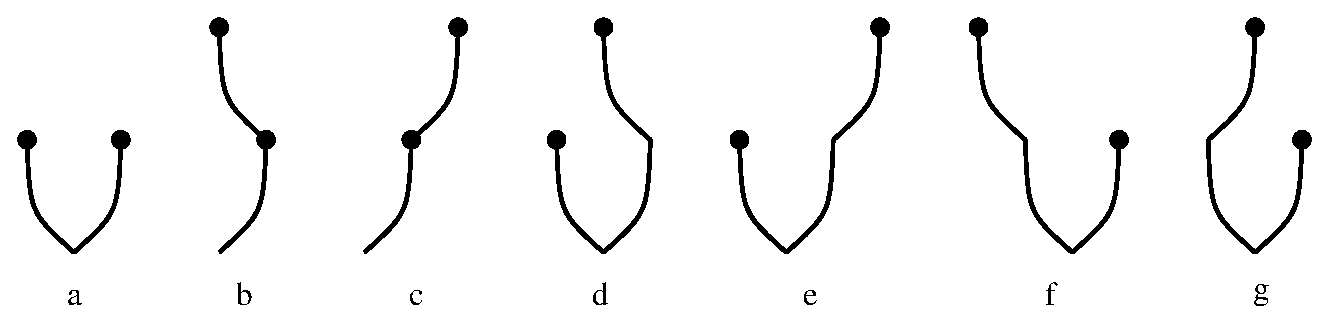
\includegraphics[scale=0.5]{embTypeExamples.eps}
%  \centering \includegraphics[scale=0.4]{figures/embType3Branching.pdf}
%  \caption{
%    Another set of different embedding types, in a more branching underlying tree. % , by their smallest representative, a strong subtree
%    All of them are again different.
%  }
%  \label{fig:some-emb-types-3-branching}
%\end{figure}

\begin{figure}[h]
%  \centering 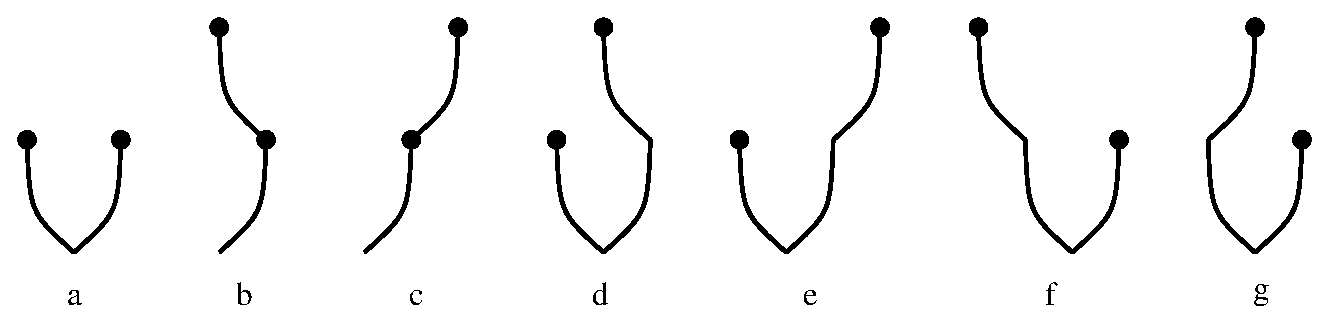
\includegraphics[scale=0.5]{embTypeExamples.eps}
  \centering
  %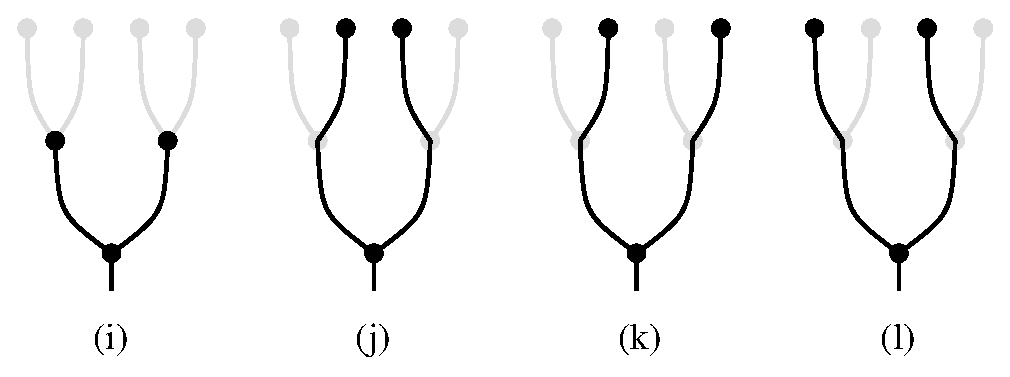
\includegraphics[scale=0.4]{figures/sameEmbdedingTypes.eps}
  \begin{tikzpicture}[scale=1.5,font=\footnotesize]
		\tikzset{
			empty node/.style={circle,inner sep=0,fill=none},
			solid node/.style={circle,draw,inner sep=1.5,fill=black},
			hollow node/.style={circle,draw,inner sep=1.5,fill=white},
			gray node/.style={circle,draw={rgb:black,1;white,4},inner sep=1.5,fill={rgb:black,1;white,4}}
		}
		\tikzset{snake it/.style={decorate, decoration=snake, line cap=round}}
		\tikzset{gray line/.style={line cap=round,thick,color={rgb:black,1;white,4}}}
		\tikzset{thick line/.style={line cap=round,rounded corners=0.1mm,thick}}
		\node (a)[solid node] at (0,0) {};
		\node (a1)[solid node] at (0.3,0.5) {};
		\node (a0)[solid node] at (-0.3,0.5) {};
		\node (a00)[gray node] at (-0.45,1) {};
		\node (a01)[gray node] at (-0.15,1) {};
		\node (a10)[gray node] at (0.15,1) {};
		\node (a11)[gray node] at (0.45,1) {};
		\begin{pgfonlayer}{background}
		\draw[-,thick line] (a) to (a0);
		\draw[-,thick line] (a) to (a1);
		\draw[-,gray line] (a0) to (a00);
		\draw[-,gray line] (a0) to (a01);
		\draw[-,gray line] (a1) to (a10);
		\draw[-,gray line] (a1) to (a11);
		\end{pgfonlayer}
		\node at (0,-0.5) {(i)};
	\end{tikzpicture}
	\hspace{5mm}
	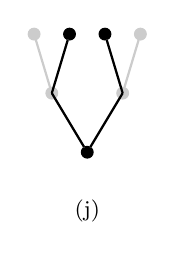
\begin{tikzpicture}[scale=1.5,font=\footnotesize]
		\tikzset{
			empty node/.style={circle,inner sep=0,fill=none},
			solid node/.style={circle,draw,inner sep=1.5,fill=black},
			hollow node/.style={circle,draw,inner sep=1.5,fill=white},
			gray node/.style={circle,draw={rgb:black,1;white,4},inner sep=1.5,fill={rgb:black,1;white,4}}
		}
		\tikzset{snake it/.style={decorate, decoration=snake, line cap=round}}
		\tikzset{gray line/.style={line cap=round,thick,color={rgb:black,1;white,4}}}
		\tikzset{thick line/.style={line cap=round,rounded corners=0.1mm,thick}}
		\node (a)[solid node] at (0,0) {};
		\node (a1)[gray node] at (0.3,0.5) {};
		\node (a0)[gray node] at (-0.3,0.5) {};
		\node (a00)[gray node] at (-0.45,1) {};
		\node (a01)[solid node] at (-0.15,1) {};
		\node (a10)[solid node] at (0.15,1) {};
		\node (a11)[gray node] at (0.45,1) {};
		\draw[-,gray line] (a) to (a0);
		\draw[-,gray line] (a) to (a1);
		\draw[-,gray line] (a0) to (a00);
		\draw[-,gray line] (a0) to (a01);
		\draw[-,gray line] (a1) to (a10);
		\draw[-,gray line] (a1) to (a11);
		\draw[-,thick line] (a) to (0.3,0.5) to (a10);
		\draw[-,thick line] (a) to (-0.3,0.5) to (a01);
		\node at (0,-0.5) {(j)};
	\end{tikzpicture}
	\hspace{5mm}
	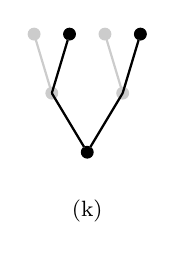
\begin{tikzpicture}[scale=1.5,font=\footnotesize]
		\tikzset{
			empty node/.style={circle,inner sep=0,fill=none},
			solid node/.style={circle,draw,inner sep=1.5,fill=black},
			hollow node/.style={circle,draw,inner sep=1.5,fill=white},
			gray node/.style={circle,draw={rgb:black,1;white,4},inner sep=1.5,fill={rgb:black,1;white,4}}
		}
		\tikzset{snake it/.style={decorate, decoration=snake, line cap=round}}
		\tikzset{gray line/.style={line cap=round,thick,color={rgb:black,1;white,4}}}
		\tikzset{thick line/.style={line cap=round,rounded corners=0.1mm,thick}}
		\node (a)[solid node] at (0,0) {};
		\node (a1)[gray node] at (0.3,0.5) {};
		\node (a0)[gray node] at (-0.3,0.5) {};
		\node (a00)[gray node] at (-0.45,1) {};
		\node (a01)[solid node] at (-0.15,1) {};
		\node (a10)[gray node] at (0.15,1) {};
		\node (a11)[solid node] at (0.45,1) {};
		\draw[-,gray line] (a) to (a0);
		\draw[-,gray line] (a) to (a1);
		\draw[-,gray line] (a0) to (a00);
		\draw[-,gray line] (a0) to (a01);
		\draw[-,gray line] (a1) to (a10);
		\draw[-,gray line] (a1) to (a11);
		\draw[-,thick line] (a) to (0.3,0.5) to (a11);
		\draw[-,thick line] (a) to (-0.3,0.5) to (a01);
		\node at (0,-0.5) {(k)};
	\end{tikzpicture}
	\hspace{5mm}
	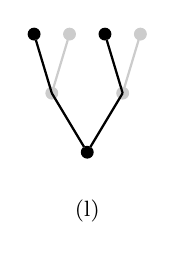
\begin{tikzpicture}[scale=1.5,font=\footnotesize]
		\tikzset{
			empty node/.style={circle,inner sep=0,fill=none},
			solid node/.style={circle,draw,inner sep=1.5,fill=black},
			hollow node/.style={circle,draw,inner sep=1.5,fill=white},
			gray node/.style={circle,draw={rgb:black,1;white,4},inner sep=1.5,fill={rgb:black,1;white,4}}
		}
		\tikzset{snake it/.style={decorate, decoration=snake, line cap=round}}
		\tikzset{gray line/.style={line cap=round,thick,color={rgb:black,1;white,4}}}
		\tikzset{thick line/.style={line cap=round,rounded corners=0.1mm,thick}}
		\node (a)[solid node] at (0,0) {};
		\node (a1)[gray node] at (0.3,0.5) {};
		\node (a0)[gray node] at (-0.3,0.5) {};
		\node (a00)[solid node] at (-0.45,1) {};
		\node (a01)[gray node] at (-0.15,1) {};
		\node (a10)[solid node] at (0.15,1) {};
		\node (a11)[gray node] at (0.45,1) {};
		\draw[-,gray line] (a) to (a0);
		\draw[-,gray line] (a) to (a1);
		\draw[-,gray line] (a0) to (a00);
		\draw[-,gray line] (a0) to (a01);
		\draw[-,gray line] (a1) to (a10);
		\draw[-,gray line] (a1) to (a11);
		\draw[-,thick line] (a) to (-0.3,0.5) to (a00);
		\draw[-,thick line] (a) to (0.3,0.5) to (a10);
		\node at (0,-0.5) {(l)};
	\end{tikzpicture}
  \caption{
    A few finite level-closed subtrees with the same embedding type. The fact that they are level-closed depends on the underlying grey tree.
  }
  \label{fig:same-emb-types}
\end{figure}

\begin{figure}[h]
%  \centering 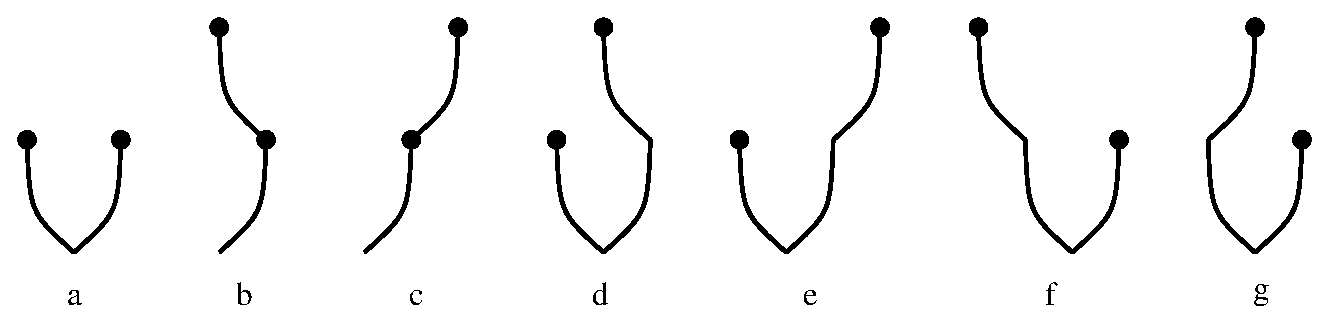
\includegraphics[scale=0.5]{embTypeExamples.eps}
  \centering
     % \input{figures/someHeight.pdf_t}
	\begin{tikzpicture}[scale=1.5,font=\footnotesize]
		\tikzset{
			empty node/.style={circle,inner sep=0,fill=none},
			solid node/.style={circle,draw,inner sep=1.5,fill=black},
			hollow node/.style={circle,draw,inner sep=1.5,fill=white},
			gray node/.style={circle,draw={rgb:black,1;white,4},inner sep=1.5,fill={rgb:black,1;white,4}}
		}
		\tikzset{snake it/.style={decorate, decoration=snake, line cap=round}}
		\tikzset{gray line/.style={line cap=round,thick,color={rgb:black,1;white,4}}}
		\tikzset{thick line/.style={line cap=round,rounded corners=0.1mm,thick}}
		\node (a)[gray node] at (0-0.6,0) {};
		\node (a1)[gray node] at (0.3-0.6,0.5) {};
		\node (a0)[solid node] at (-0.3-0.6,0.5) {};
		\node (a00)[gray node] at (-0.45-0.6,1) {};
		\node (a01)[gray node] at (-0.15-0.6,1) {};
		\node (a10)[gray node] at (0.15-0.6,1) {};
		\node (a11)[gray node] at (0.45-0.6,1) {};
		\draw[-,thick line] (0-0.6,0) to (a0);
		\draw[-,gray line] (a) to (a1);
		\begin{pgfonlayer}{background}
		\draw[-,gray line] (a0) to (a00);
		\draw[-,gray line] (a0) to (a01);
		\end{pgfonlayer}
		\draw[-,gray line] (a1) to (a10);
		\draw[-,gray line] (a1) to (a11);
		\node (b)[solid node] at (0+0.6,0) {};
		\node (b1)[gray node] at (0.3+0.6,0.5) {};
		\node (b0)[gray node] at (-0.3+0.6,0.5) {};
		\node (b00)[gray node] at (-0.45+0.6,1) {};
		\node (b01)[gray node] at (-0.15+0.6,1) {};
		\node (b10)[gray node] at (0.15+0.6,1) {};
		\node (b11)[gray node] at (0.45+0.6,1) {};
		\begin{pgfonlayer}{background}
		\draw[-,gray line] (b) to (b0);
		\draw[-,gray line] (b) to (b1);
		\draw[-,gray line] (b0) to (b00);
		\draw[-,gray line] (b0) to (b01);
		\draw[-,gray line] (b1) to (b10);
		\draw[-,gray line] (b1) to (b11);
		\end{pgfonlayer}
		\node at (0,-0.5) {height 1};
	\end{tikzpicture}
	\hspace{5mm}
	\begin{tikzpicture}[scale=1.5,font=\footnotesize]
		\tikzset{
			empty node/.style={circle,inner sep=0,fill=none},
			solid node/.style={circle,draw,inner sep=1.5,fill=black},
			hollow node/.style={circle,draw,inner sep=1.5,fill=white},
			gray node/.style={circle,draw={rgb:black,1;white,4},inner sep=1.5,fill={rgb:black,1;white,4}}
		}
		\tikzset{snake it/.style={decorate, decoration=snake, line cap=round}}
		\tikzset{gray line/.style={line cap=round,thick,color={rgb:black,1;white,4}}}
		\tikzset{thick line/.style={line cap=round,rounded corners=0.1mm,thick}}
		\node (a)[solid node] at (0-0.6,0) {};
		\node (a1)[gray node] at (0.3-0.6,0.5) {};
		\node (a0)[gray node] at (-0.3-0.6,0.5) {};
		\node (a00)[gray node] at (-0.45-0.6,1) {};
		\node (a01)[solid node] at (-0.15-0.6,1) {};
		\node (a10)[gray node] at (0.15-0.6,1) {};
		\node (a11)[solid node] at (0.45-0.6,1) {};
		\draw[-,thick line] (a) to (-0.3-0.6,0.5) to (a01);
		\draw[-,thick line] (a) to (0.3-0.6,0.5) to (a11);
		\draw[-,gray line] (a0) to (a00);
		\draw[-,gray line] (a1) to (a10);
		\node (b)[solid node] at (0+0.6,0) {};
		\node (b1)[solid node] at (0.3+0.6,0.5) {};
		\node (b0)[solid node] at (-0.3+0.6,0.5) {};
		\node (b00)[gray node] at (-0.45+0.6,1) {};
		\node (b01)[gray node] at (-0.15+0.6,1) {};
		\node (b10)[gray node] at (0.15+0.6,1) {};
		\node (b11)[gray node] at (0.45+0.6,1) {};
		\begin{pgfonlayer}{background}
		\draw[-,thick line] (b) to (b0);
		\draw[-,thick line] (b) to (b1);
		\draw[-,gray line] (b0) to (b00);
		\draw[-,gray line] (b0) to (b01);
		\draw[-,gray line] (b1) to (b10);
		\draw[-,gray line] (b1) to (b11);
		\end{pgfonlayer}
		\node at (0,-0.5) {height 2};
	\end{tikzpicture}
	\hspace{5mm}
	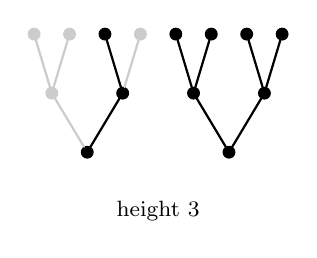
\begin{tikzpicture}[scale=1.5,font=\footnotesize]
		\tikzset{
			empty node/.style={circle,inner sep=0,fill=none},
			solid node/.style={circle,draw,inner sep=1.5,fill=black},
			hollow node/.style={circle,draw,inner sep=1.5,fill=white},
			gray node/.style={circle,draw={rgb:black,1;white,4},inner sep=1.5,fill={rgb:black,1;white,4}}
		}
		\tikzset{snake it/.style={decorate, decoration=snake, line cap=round}}
		\tikzset{gray line/.style={line cap=round,thick,color={rgb:black,1;white,4}}}
		\tikzset{thick line/.style={line cap=round,rounded corners=0.1mm,thick}}
		\node (a)[solid node] at (0-0.6,0) {};
		\node (a1)[solid node] at (0.3-0.6,0.5) {};
		\node (a0)[gray node] at (-0.3-0.6,0.5) {};
		\node (a00)[gray node] at (-0.45-0.6,1) {};
		\node (a01)[gray node] at (-0.15-0.6,1) {};
		\node (a10)[solid node] at (0.15-0.6,1) {};
		\node (a11)[gray node] at (0.45-0.6,1) {};
		\draw[-,gray line] (a) to (a0);
		\draw[-,thick line] (a) to (a1);
		\draw[-,gray line] (a0) to (a00);
		\draw[-,gray line] (a0) to (a01);
		\draw[-,thick line] (a1) to (a10);
		\draw[-,gray line] (a1) to (a11);
		\node (b)[solid node] at (0+0.6,0) {};
		\node (b1)[solid node] at (0.3+0.6,0.5) {};
		\node (b0)[solid node] at (-0.3+0.6,0.5) {};
		\node (b00)[solid node] at (-0.45+0.6,1) {};
		\node (b01)[solid node] at (-0.15+0.6,1) {};
		\node (b10)[solid node] at (0.15+0.6,1) {};
		\node (b11)[solid node] at (0.45+0.6,1) {};
		\draw[-,thick line] (b) to (b0);
		\draw[-,thick line] (b) to (b1);
		\draw[-,thick line] (b0) to (b00);
		\draw[-,thick line] (b0) to (b01);
		\draw[-,thick line] (b1) to (b10);
		\draw[-,thick line] (b1) to (b11);
		\node at (0,-0.5) {height 3};
	\end{tikzpicture}
%      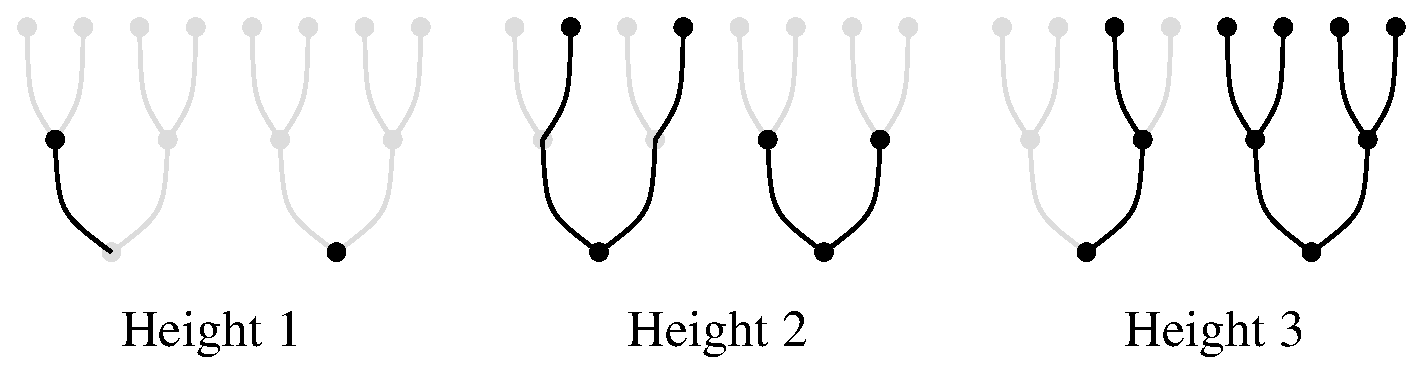
\includegraphics[scale=0.4]{figures/someHeight.eps}
  \caption{ Some subtrees with embedding type of different height. The two first have the same embedding type, the unique embedding type of height 1. The two in the middle have the same embedding type, of height 2. The last pair consists of level-closed subtrees with two different embedding types of height 3. }
  \label{fig:some-emb-height}
\end{figure}


%\begin{definition}
%If $\embfont e$ is an embedding type, and $T$ a tree, then \[\Subtree{\embfont e}{T}=\{F\subseteq T: F\text{ has embedding type $\embfont e$ in $T$}\}\]
%\end{definition}
%We already emphasized the fact that embedding types are a relative notion to a parent tree, this has the effect that in general, if $S$ is a subtree of $T$ and $\embfont e$ is an embedding type, then $\Subtree{\embfont e}{S}$ might not be included in  $\Subtree{\embfont e}{T}$. However, if $S$ is a strong subtree of $T$, then $\Subtree{\embfont e}{S}\subseteq\Subtree{\embfont e}{T}$. In \Cref{fig:same-emb-types,fig:some-emb-height,fig:some-emb-types}, we illustrate the notion of embedding types for subtrees of $\cantor$.

%\section{Binary trees and embedding types}
%Our primary focus will be on infinite perfect binary trees.
%
%\begin{definition}
%  A \emph{binary tree} is a tree $T\subseteq\cantor$. A tree $T$ is \emph{perfect} if it is binary and every node is either $2$-branching or a leaf, and all leaves are at the same level and no $2$-branching node and leaf are at the same level. An embedding type $\embfont e$ is \emph{binary} if it is the embedding type of a subtree of binary tree, that is, $\Subtree{\embfont e}{T}$ for some binary tree $T$.
%\end{definition}
%In the case of a binary tree,  every branching node is
%at most 2-branching, moreover it branches immediately, that is for every
%$\sigma\in T$, letting  $\tau_0,\tau_1\in T$ be the two immediate successors of
%$\sigma$ in $T$, $\sigma\cat0\preceq\tau_0$ and
%$\sigma\cat1\preceq\tau_1$. Indeed, suppose for the contradiction that, say, $\sigma\cat0\preceq\tau_0$ and $\sigma\cat0\preceq\tau_1$.Then by definition of a tree, $\tau_0\meet_T\tau_1 \in T$, but then $\sigma\cat0 \prec \tau_0\meet_T\tau_1$, contradicting the fact that $\tau_0$ and $\tau_1$ are immediate successors of $\sigma$ in $T$.
%
%This definition slightly differs from the standard definition of a binary tree in computability theory, in which the trees are closed under prefixes. In this definition, a weaker downward closure is specified: the only prefixes of a node that need to be in the trees are the immediately splitting one.
%
%A perfect tree is infinite if and only if it has no leaf. Unless specified, we will consider only infinite perfect trees.
%A perfect tree might not be a strong subtree of $\cantor$, by failure of \Cref{pt:preserve-levels} of \Cref{def:strong-subtree}.
%
%Perfect trees have the nice property that they have a member of every binary embedding type. Therefore, a strong subtree $S$ of a perfect binary tree $T$ also has this property, and as it preserves embedding types, $\Subtree{\embfont e}{T}\cap \Subtree{\embfont e}S\neq\emptyset$ for any binary embedding type $\embfont e$.
%
%Figure~\ref{fig:some-emb-types} is a visual
%representation of some embedding types. Figure~\ref{fig:same-emb-types} is a collection of different subtrees with the same embedding type.
%
%The reason we are most interested in binary tree is that for every $n$, there exists a ``strongest'' embedding type $\embfont e^n$, in the sense that Milliken's tree theorem for binary tree and embedding type of height $n$ can be reduced to the result for this particular embedding type $\embfont e^n$  (see
%Remark~\ref{rem:milli-for-ntuple}). We will therefore focus on the following
%embedding types. The reason for this is that if $T$ is a perfect binary tree, $\embfont e$ is a binary embedding type of height $n$ and $F\in\Subtree{\embfont e}{T}$, then there exists $G\subseteq T$ such that $F\cup G\in\Subtree{\embfont e^n}{T}$, that is $F$ can be completed to have embedding type $\embfont e^n$. This completion cannot always occur in binary trees that are not perfect.
%\begin{definition}
%  We call $\embtype{n}$ the embedding type of the subtree $2^{<n}$ of $\cantor$.
%\end{definition}
%For instance, the embedding type (h) of Figure~\ref{fig:some-emb-types} is $\embfont e_3$.
%
%\begin{remark}\label{rem:milli-for-ntuple}
%  In the case of perfect binary trees, Milliken's tree theorem for height $n$ follows from its restriction to the embedding type $\embtype{n}$. Indeed, if $\embfont e$ is a binary embedding
%  type of height $n$, then a coloring of
%  $\Subtree{\embfont e}{T}$ induces a coloring of
%  $\Subtree{\embtype{n}}{T}$ by ``forgetting'' the additional
%  branches in $\embtype{n}$. For instance, if $\embfont e$ is
%    the embedding type of $\{\emptystr,0\}$, that is the coloring $f$
%    is defined on pairs of strings $\sigma, \tau$ with
%    $\sigma\cat0\prec\tau$, then we define
%    $g(\{\sigma,\sigma\cat0\cat\tau_0,\sigma\cat1\cat\tau_1\})$ to be
%    $f(\{\sigma,\sigma\cat0\cat\tau_0\})$. Any solution given by
%  $\MT n{}$ for this induced coloring is a solution for the initial
%  coloring.
%\end{remark}

%\section{Definitions and notations}
%
%For this section, the trees we consider will always be binary trees. For this section we also consider that trees are in general not necessarily meet closed: A tree is simply a non-empty set of strings of $2^{<\omega}$. When a tree is meet-closed we will then specify it explicitly. A node $\sigma \in T$ for a tree $T$ is branching if it has two incomparable immediate extensions. An infinite tree is \emph{perfect} if each of its node is branching. A finite tree $T$ is said to be perfect if each of its node is either a leaf or branching. 
%
%\begin{definition}
%Given two trees $S_1,S_2 \subseteq 2^{<\omega}$, a function $f:S_1 \rightarrow S_2$ is an \emph{isomorphism} if it is a bijection, if $\sigma \preceq \tau$ iff $f(\sigma) \preceq f(\tau)$ and if $\sigma \leq_L \tau$ iff $f(\sigma) \leq_L f(\tau)$ where $\leq_L$ is the lexicographic order.
%\end{definition}
%
%Note that a tree $T$ is perfect iff there is an isomorphism $f:2^{<\omega} \rightarrow T$. Recall that given a strong subtree $T \subseteq 2^{<\omega}$ and given $S \subseteq T$, the strong closure of $S$ inside $T$, denoted by $S^{cl}$ equals $(S^{\wedge})^{lvl}$. Note that $S^{cl}$ is always the smallest strong perfect subtree of $T$ containing $S$.
%
%\begin{definition}
%Given two strong subtree $S_1,S_2 \subseteq 2^{<\omega}$, a function $f:S_1 \rightarrow S_2$ is a \emph{strong isomorphism} if it is a bijection and if for $\sigma_1,\sigma_2 \in S$ we have $\sigma_1 i \preceq \sigma_2$ iff $f(\sigma_1) i \preceq f(\sigma_2)$ for $i \in \{0,1\}$.
%\end{definition}
%
%Recall that embedding types are equivalence classes under strong isomorphisms. Also given
%
%a tuple $\overline{\sigma} \in [2^{<\omega}]^n$, the embedding type generated by $\overline{\sigma}$ is given by the equivalence class of $\overline{\sigma}^{cl}$.


\section{Strong generalized CHM tree theorem}

No embedding type can be avoided in a strong subtree of $2^{<\omega}$. For this reason the number of colors that cannot be avoided by $n$-tuples of elements of $2^{<\omega}$ is at least the number of embedding types that can be generated by these tuples.

\begin{definition}\index{$e_{\sTT}$}
Let $e_{\sTT}:\omega \rightarrow \omega$ be the function which to $n$ associates the number of embedding types that can be generated by $n$ distinct strings. 
\end{definition}

Let us provide an example with \Cref{fig:tuple-to-height}: all the possible embedding types that are generated by two strings. We have $e_{\sTT}(2) = 7$.

\begin{figure}[h]
  \begin{center}
   % \includegraphics[scale=0.5]{figures/embTypeGeneratedBy2Nodes.pdf}\\
    \begin{tikzpicture}[scale=1.5,font=\footnotesize]
		\tikzset{
			empty node/.style={circle,inner sep=0,fill=none},
			solid node/.style={circle,draw,inner sep=1.5,fill=black},
			hollow node/.style={circle,draw,inner sep=1.5,fill=white},
			gray node/.style={circle,draw={rgb:black,1;white,4},inner sep=1.5,fill={rgb:black,1;white,4}}
		}
		\tikzset{snake it/.style={decorate, decoration=snake, line cap=round}}
		\tikzset{gray line/.style={line cap=round,thick,color={rgb:black,1;white,4}}}
		\tikzset{thick line/.style={line cap=round,rounded corners=0.1mm,thick}}
		\begin{pgfonlayer}{background}
		\node (a)[solid node] at (0,0) {};
		\node (a1)[solid node] at (0.3,0.5) {};
		\node (a0)[solid node] at (-0.3,0.5) {};
		\draw[fill=none] (a0) circle [radius=0.75mm];
		\draw[fill=none] (a1) circle [radius=0.75mm];
		\end{pgfonlayer}
		\draw[-,thick line] (a) to (a0);
		\draw[-,thick line] (a) to (a1);
	\end{tikzpicture}
	\hspace{5mm}
	\begin{tikzpicture}[scale=1.5,font=\footnotesize]
		\tikzset{
			empty node/.style={circle,inner sep=0,fill=none},
			solid node/.style={circle,draw,inner sep=1.5,fill=black},
			hollow node/.style={circle,draw,inner sep=1.5,fill=white},
			gray node/.style={circle,draw={rgb:black,1;white,4},inner sep=1.5,fill={rgb:black,1;white,4}}
		}
		\tikzset{snake it/.style={decorate, decoration=snake, line cap=round}}
		\tikzset{gray line/.style={line cap=round,thick,color={rgb:black,1;white,4}}}
		\tikzset{thick line/.style={line cap=round,rounded corners=0.1mm,thick}}
		\begin{pgfonlayer}{background}
		\node (a)[solid node] at (0,0) {};
		\node (a1)[solid node] at (0.3,0.5) {};
		\draw[fill=none] (a) circle [radius=0.75mm];
		\draw[fill=none] (a1) circle [radius=0.75mm];
		\end{pgfonlayer}
		\draw[-,thick line] (a) to (a1);
	\end{tikzpicture}
	\hspace{5mm}
	\begin{tikzpicture}[scale=1.5,font=\footnotesize]
		\tikzset{
			empty node/.style={circle,inner sep=0,fill=none},
			solid node/.style={circle,draw,inner sep=1.5,fill=black},
			hollow node/.style={circle,draw,inner sep=1.5,fill=white},
			gray node/.style={circle,draw={rgb:black,1;white,4},inner sep=1.5,fill={rgb:black,1;white,4}}
		}
		\tikzset{snake it/.style={decorate, decoration=snake, line cap=round}}
		\tikzset{gray line/.style={line cap=round,thick,color={rgb:black,1;white,4}}}
		\tikzset{thick line/.style={line cap=round,rounded corners=0.1mm,thick}}
		\begin{pgfonlayer}{background}
		\node (a)[solid node] at (0,0) {};
		\node (a0)[solid node] at (-0.3,0.5) {};
		\draw[fill=none] (a) circle [radius=0.75mm];
		\draw[fill=none] (a0) circle [radius=0.75mm];
		\end{pgfonlayer}
		\draw[-,thick line] (a) to (a0);
	\end{tikzpicture}
	\hspace{5mm}
	\begin{tikzpicture}[scale=1.5,font=\footnotesize]
		\tikzset{
			empty node/.style={circle,inner sep=0,fill=none},
			solid node/.style={circle,draw,inner sep=1.5,fill=black},
			hollow node/.style={circle,draw,inner sep=1.5,fill=white},
			gray node/.style={circle,draw={rgb:black,1;white,4},inner sep=1.5,fill={rgb:black,1;white,4}}
		}
		\tikzset{snake it/.style={decorate, decoration=snake, line cap=round}}
		\tikzset{gray line/.style={line cap=round,thick,color={rgb:black,1;white,4}}}
		\tikzset{thick line/.style={line cap=round,rounded corners=0.1mm,thick}}
		\begin{pgfonlayer}{background}
		\node (a)[solid node] at (0,0) {};
		\node (a1)[solid node] at (0.3,0.5) {};
		\node (a0)[solid node] at (-0.3,0.5) {};
		\node (a10)[solid node] at (0.15,1) {};
		\draw[fill=none] (a0) circle [radius=0.75mm];
		\draw[fill=none] (a10) circle [radius=0.75mm];
		\end{pgfonlayer}
		\draw[-,thick line] (a) to (a0);
		\draw[-,thick line] (a) to (a1);
		\draw[-,thick line] (a1) to (a10);
	\end{tikzpicture}
	\hspace{5mm}
	\begin{tikzpicture}[scale=1.5,font=\footnotesize]
		\tikzset{
			empty node/.style={circle,inner sep=0,fill=none},
			solid node/.style={circle,draw,inner sep=1.5,fill=black},
			hollow node/.style={circle,draw,inner sep=1.5,fill=white},
			gray node/.style={circle,draw={rgb:black,1;white,4},inner sep=1.5,fill={rgb:black,1;white,4}}
		}
		\tikzset{snake it/.style={decorate, decoration=snake, line cap=round}}
		\tikzset{gray line/.style={line cap=round,thick,color={rgb:black,1;white,4}}}
		\tikzset{thick line/.style={line cap=round,rounded corners=0.1mm,thick}}
		\begin{pgfonlayer}{background}
		\node (a)[solid node] at (0,0) {};
		\node (a1)[solid node] at (0.3,0.5) {};
		\node (a0)[solid node] at (-0.3,0.5) {};
		\node (a11)[solid node] at (0.45,1) {};
		\draw[fill=none] (a0) circle [radius=0.75mm];
		\draw[fill=none] (a11) circle [radius=0.75mm];
		\end{pgfonlayer}
		\draw[-,thick line] (a) to (a0);
		\draw[-,thick line] (a) to (a1);
		\draw[-,thick line] (a1) to (a11);
	\end{tikzpicture}
	\hspace{5mm}
	\begin{tikzpicture}[scale=1.5,font=\footnotesize]
		\tikzset{
			empty node/.style={circle,inner sep=0,fill=none},
			solid node/.style={circle,draw,inner sep=1.5,fill=black},
			hollow node/.style={circle,draw,inner sep=1.5,fill=white},
			gray node/.style={circle,draw={rgb:black,1;white,4},inner sep=1.5,fill={rgb:black,1;white,4}}
		}
		\tikzset{snake it/.style={decorate, decoration=snake, line cap=round}}
		\tikzset{gray line/.style={line cap=round,thick,color={rgb:black,1;white,4}}}
		\tikzset{thick line/.style={line cap=round,rounded corners=0.1mm,thick}}
		\begin{pgfonlayer}{background}
		\node (a)[solid node] at (0,0) {};
		\node (a1)[solid node] at (0.3,0.5) {};
		\node (a0)[solid node] at (-0.3,0.5) {};
		\node (a00)[solid node] at (-0.45,1) {};
		\draw[fill=none] (a1) circle [radius=0.75mm];
		\draw[fill=none] (a00) circle [radius=0.75mm];
		\end{pgfonlayer}
		\draw[-,thick line] (a) to (a0);
		\draw[-,thick line] (a) to (a1);
		\draw[-,thick line] (a0) to (a00);
	\end{tikzpicture}
	\hspace{5mm}
	\begin{tikzpicture}[scale=1.5,font=\footnotesize]
		\tikzset{
			empty node/.style={circle,inner sep=0,fill=none},
			solid node/.style={circle,draw,inner sep=1.5,fill=black},
			hollow node/.style={circle,draw,inner sep=1.5,fill=white},
			gray node/.style={circle,draw={rgb:black,1;white,4},inner sep=1.5,fill={rgb:black,1;white,4}}
		}
		\tikzset{snake it/.style={decorate, decoration=snake, line cap=round}}
		\tikzset{gray line/.style={line cap=round,thick,color={rgb:black,1;white,4}}}
		\tikzset{thick line/.style={line cap=round,rounded corners=0.1mm,thick}}
		\begin{pgfonlayer}{background}
		\node (a)[solid node] at (0,0) {};
		\node (a1)[solid node] at (0.3,0.5) {};
		\node (a0)[solid node] at (-0.3,0.5) {};
		\node (a01)[solid node] at (-0.15,1) {};
		\draw[fill=none] (a1) circle [radius=0.75mm];
		\draw[fill=none] (a01) circle [radius=0.75mm];
		\end{pgfonlayer}
		\draw[-,thick line] (a) to (a0);
		\draw[-,thick line] (a) to (a1);
		\draw[-,thick line] (a0) to (a01);
	\end{tikzpicture}
    \caption{The seven possible embedding types generated by two nodes (shown as circled). That is, these are the embedding types of their full closure. The maximal height of the embedding types here is 3.}
     \label{fig:tuple-to-height}
\end{center}
\end{figure}

Given an element of $[2^{<\omega}]^n$ one can computably recognize which embedding type it generates. It follows that given an enumeration $\embfont e_1, \embfont e_2, \dots, \embfont e_{e_{\sTT}(n)}$ of the embedding types that can be generated by $n$ distinct strings, one can define the color $c$ on $[2^{<\omega}]^n$ which to each element generating the embedding type $\embfont e_i$ associates $i$. No strong subtree of $2^{<\omega}$ can avoid any embedding type and thus at least $e_{\sTT}(n)$ colors are used by $c$ within any strong subtree of $2^{<\omega}$.

We can in fact force even more colors: Given a finite strong subtree $F \subseteq 2^{<\omega}$, there might be distinct tuples $\overline{\sigma_1},\overline{\sigma_2} \in [F]^n$ such that $\overline{\sigma_1}^{cl} = \overline{\sigma_2}^{cl} = F$. Note that such a phenomenon does not happen for $n=2$ and below, but start to happen from $n=3$. For instance the tuples $\{\sigma0,\sigma1,\sigma00\}$ and $\{\sigma,\sigma1,\sigma00\}$ generate the same embedding type. This leads to the following definition:

\begin{definition}\index{tuple type}\index{type!tuple}
A \emph{tuple type} is an equivalence class on the following relation defined on $\bigcup_n [2^{<\omega}]^n \times [2^{<\omega}]^n$: We say that $\overline{\sigma}, \overline{\tau} \in [2^{<\omega}]^n$ are equivalent if there is a strong isomorphism $f$ from $\overline{\sigma}^{\mathrm{cl}}$ to $\overline{\tau}^{\mathrm{cl}}$ which associates elements of $\overline{\sigma}$ to elements of $\overline{\tau}$.
\end{definition}

Note that the tuple types are a refinement of the embedding types. Also for $n>2$ this refinement is strict, by the example given above with $\{\sigma0,\sigma1,\sigma00\}$ and $\{\sigma,\sigma1,\sigma00\}$: no strong isomorphism from $\{\sigma0,\sigma1,\sigma00\}^{\mathrm{cl}}$ to $\{\sigma,\sigma1,\sigma00\}^{\mathrm{cl}}$ can map elements of $\{\sigma0,\sigma1,\sigma00\}$ to elements of $\{\sigma,\sigma1,\sigma00\}$ as no string is a prefix of the other two in the former but one is in the latter.

\begin{definition}\index{$t_{\sTT}$}
Let $t_{\sTT}:\omega \rightarrow \omega$ be the function which to $n$ associates the number of tuple types that can be generated by $n$ distinct strings. 
\end{definition}

Just like a coloring on $[2^{<\omega}]^n$ can recognize the generated embedding types, it can recognize the corresponding tuple types: the embedding type together with the role played by each string generating it. And just like no embedding type can be avoided in a strong perfect tree, also no tuple type can be avoided in a strong perfect tree. It follows that if $c$ is a coloring of $[2^{<\omega}]^n$ which associates to an element its corresponding tuple type, then any strong perfect subtree of $T$ needs at least $t_{\sTT}(n)$ colors. In the next section we show that this number is optimal.

% \begin{definition}
%   The statement ``strong generalized tree theorem'' is the following statement: ``for every coloring $f:[\cantor]^n\to l$, there exists a perfect tree $T$ such that $[T]^n$ uses at most $k$ color''...

%   The statement ``strong generalized tree theorem'' is the following statement: ``for every coloring $f:[\cantor]^n\to l$, there exists a perfect tree $T$ such that $[T]^n$ uses at most $k$ color''...
% \end{definition}

We are now ready to formally state and prove the strong generalized CHM tree theorem.

\begin{theorem}[Strong generalized CHM tree theorem] \label{th:strong_gen_treeth}
For every $n$, the principle $(\forall k) \mathrm{SCMHTT^n_{k,t_{\sTT}(n)}}$ is provable in $\ACA_0$, and $\RCA_0$ proves that the principle $(\forall k) \mathrm{SCMHTT^n_{k,t_{\sTT}(n)-1}}$ is false.
\end{theorem}
\begin{proof}
We already saw that this principle is false when the maximal number of color is $t_{\sTT}(n)-1$, with as an example the coloring on $[2^{<\omega}]^n$ which on each element associates an integer representing its tuple type.

Let us now show that one can prove the statement within $\ACA_0$ for $t_{\sTT}(n)$ colors. Let $\embfont t_1, \embfont t_2, \dots, \embfont t_{t_{\sTT}(n)}$ be an enumeration of the tuple types of size $n$. Let $c$ be any coloring on the elements of $[2^{<\omega}]^n$.

%Let us fix a model $\Mc$ of $\ACA_0$, and a finite coloring $c \in \Mc$ of $[2^{<\omega}]^n$. From \Cref{Th:milliken_aca}, given any strong perfect subtree $T \subseteq 2^{<\omega}$ which belongs to $\Mc$, given any embedding type $\embfont e$ and given any coloring $d:[T]^{\embfont e}$ which belongs to  $\Mc$, there exists a strong perfect subtree $S \subseteq T$ which belongs to $\Mc$ and which is monochromatic for $d$.


%Note first that the theorem starts with any perfect tree $T$, note necessarily a strong subtree of $2^{<\omega}$ or not even necessarily meet closed. In this case of course the notion of embedding type is relative to $T$ and given a bijection from $T$ to $2^{<\omega}$ such that $\sigma \preceq \tau$ implies $f(\sigma) \preceq f(\tau)$ and $\sigma \leq_L \tau$ implies $f(\sigma) \leq_L f(\tau)$, we can consider that we work within $2^{<\omega}$ with the notion of strong closure and embedding types relative to $2^{<\omega}$. The strong subtree of $2^{<\omega}$ can then be pulled-back to be a strong subtree of $T$.


%We define the coloring $d \in \Mc$ on the finite strong subtrees of $2^{<\omega}$ which can be generated by elements of $[2^{<\omega}]^n$ as follow: given a finite strong subtree $F \subseteq T$ of embedding type $\embfont e_i$, let $\overline{\sigma_1}, \dots, \overline{\sigma_{k_1}}$ be all the subsets of $n$ strings of $F$ which generate $F$ (whose strong closure equals $F$). Note that we must have $j \leq k_i$. We define $d(F) = \langle c(\overline{\sigma_1}), \dots, c(\overline{\sigma_j})\rangle$. Note that $d$ is computable from $T$ and $c$ and thus $d \in \Mc$.

Let $T_0 = 2^{<\omega}$ and inductively for $i < t_{\sTT}(n)$, let $\embfont e_{i}$ be the embedding type that $\embfont t_{i}$ belongs to. Let $m_i$ be the height of the canonical representative of $\embfont t_{i}$. Let $c_i$ be the color on $T_i$ which on any strong subtree $F$ of height $m_i$ associates the color $c$ gives on the unique element of $[F]^{n}$ with tuple type $\embfont t_i$. Using \cref{thm:milliken-aca} stating that Milliken theorem for height $m_i$ is provable in $\ACA_0$, let then $T_{i+1}$ be a strong perfect subtree of $T_i$ which belongs to $\Mc$ and which is monochromatic for $c_{i}$ and let $k_{i}$ be the corresponding color. For this step, note that even if Milliken theorem is stated for strong subtrees of $2^{<\omega}$, we can also apply it for strong subtrees of $T$ where $T$ is itself a strong subtree of $2^{<\omega}$.

Let $S = T_{t_{\sTT}(n)}$. By induction we have that $S$ is a strong subtree of $2^{<\omega}$. Any $\overline{\sigma} \in [S]^n$ belongs to some tuple type $\embfont t_{i}$ and thus has color $k_i$. Thus at most $t_{\sTT}(n)$ color are used in $S$.
\end{proof}

\section{Avoiding types}

We now turn to the study of $\mathrm{CMHTT^n_{k,}}$. In particular we do not require our subtrees to be string anymore. As expected we need less colors, basically because we can avoid some embedding types, and within the embedding types which cannot be avoided, we can avoid some tuple types. 

Note that one can easily create a perfect tree which avoids almost all embedding type. Suppose we force for instance every node to be of different length. Formally such a tree has only embedding types which consists of comparable nodes, because any embedding type with two incomparable nodes contains two distinct nodes of the same length. However, this does not help: what we want is to avoid the embedding types (resp. the tuple types) which can be generated by the $n$-tuples of the tree, even though elements in the strong closure of the $n$-tuple are not necessarily all in the tree.

We will show given any strong tree $S$ how to compute a perfect subtree $T$ of $S$ which avoids as many tuple types as possible. We in fact give right away the syntactic property a tree must have to avoid as many tuple types as possible.

\begin{definition} \label{def:syntactic_minimize}\index{syntactical minimization}
We say that a perfect tree $T$ \emph{syntactically minimizes the number of tuple types} if:
\begin{enumerate}
\item[(1)] any two nodes of $T^{\wedge}$ is of different length;
\item[(2)] for any nodes $\sigma,\tau \in T$ with $\sigma \prec \tau$ we have $\sigma 0 \preceq \tau$;
\item[(3)] for any nodes $\sigma,\tau \in T^{cl}$ with $\sigma \notin T^{\wedge}$ and $\sigma \prec \tau$ we have $\sigma 0 \preceq \tau$.
\end{enumerate}
\end{definition}

Given (1), note that (3) in the previous definition is equivalent to have for any incomparable nodes $\sigma,\tau \in T^{\wedge}$ with $|\sigma| < |\tau|$ that $\tau(|\sigma|) = 0$.

\begin{lemma} \label{lem:existance_smntt}
Given any strong perfect subtree $S \subseteq 2^{<\omega}$, there is an $S$-computable perfect subtree $T \subseteq S$ which syntactically minimizes the number of tuple types.
\end{lemma}
\begin{proof}
Without loss of generality we consider that we work with $S = 2^{<\omega}$. The subtree that we build can then be pulled back in $S$ using some isomorphism between $2^{<\omega}$ and $S$.

We start by computing a meet-closed subtree $T' \subseteq 2^{\omega}$ such that (1) and (3) are satisfied. We put in $T_{0}$ the root of $2^{<\omega}$. Then inductively suppose we have a finite perfect tree $T_n$ such that each of its leaf is of level $n$ and such that for $\tau_1,\tau_2 \in T_{n}$ we have $|\tau_1| +1 < |\tau_2|$ or $|\tau_2| +1 < |\tau_1|$. Let $\sigma_1, \dots, \sigma_k$ be the leaves of $T_n$ such that $|\sigma_i|+1 < |\sigma_{i+1}|$. We define $T_{n+1, 0}$ to be $T_{n}$. Inductively for $i \leq k$ suppose we have defined a perfect tree $T_{n+1, i} \supseteq T_{n+1,0}$ such that for $\tau_1,\tau_2 \in T_{n+1, i}$ we have $|\tau_1| +1 < |\tau_2|$ or $|\tau_2| +1 < |\tau_1|$ and such that $|\sigma_i|$ is the smallest among the leaves of $T_{n+1, i}$. We let $\tau_0$ be the lexicographically smallest such that:

\begin{itemize}
\item $|\sigma_{i+1}0\tau_0| - 1$ is bigger than every string in $T_{n+1, i}$;
\item for every string $\sigma \in T_{n+1, i}$ different from $\sigma_{i+1}$ we have $\sigma_{i+1}0\tau_0(|\sigma|) = 0$. Note that by the induction hypothesis we can find such a string.
\end{itemize}
Then let $\tau_1$ be the lexicographically smallest such that:
\begin{itemize}
\item $|\sigma_{i+1}1\tau_1| - 1$ is bigger than every string in $T_{n+1, i} \cup \{\tau_0\}$;
\item for every string $\sigma \in T_{n+1, i} \cup \{\tau_0\}$ different from $\sigma_{i+1}$ we have $\sigma_{i+1}1\tau_1(|\sigma|) = 0$. Note that by the induction hypothesis we can find such a string.
\end{itemize}

Let us then define $T_{n+1, i+1} = T_{n+1, i} \cup \{\tau_0, \tau_1\}$. Note that $\sigma_{i+1}$ becomes the smallest leaf of $T_{n+1, i+1}$. Once we have defined $T_{n+1, i}$ for every $i \leq k$ we define $T_{n+1} = T_{n+1, k}$.

We finally define $T' = \bigcup_n T_n$. By construction $T'$ has the desired properties. Note that for any perfect subtree $T \subseteq T'$ then also every node is of different length, so (1) is preserved. Furthermore as $T'$ is meet closed then also for any perfect tree $T \subseteq T'$ and any two incomparable nodes $\sigma,\tau \in T^{\wedge}$ with $|\sigma| < |\tau|$ we have $\tau(|\sigma|) = 0$, so (3) is preserved.

We finally find a perfect subtree $T \subseteq T'$ such that for any $\sigma,\tau \in T$ with $\sigma \prec \tau$ we have $\sigma0 \preceq \tau$. Given an isomorphism $f:2^{<\omega}  \rightarrow T'$ we define $T$ to be the range of $f$ on strings of the form $\sigma00$ or $\sigma01$ for $\sigma \in 2^{<\omega}$. One can easily verify that $T$ is a perfect subtree of $T'$ on which (1) (2) and (3) are verified.
\end{proof}

See \Cref{fig:lastminute1} for an illustration.
\begin{figure}
	\begin{center}
	  %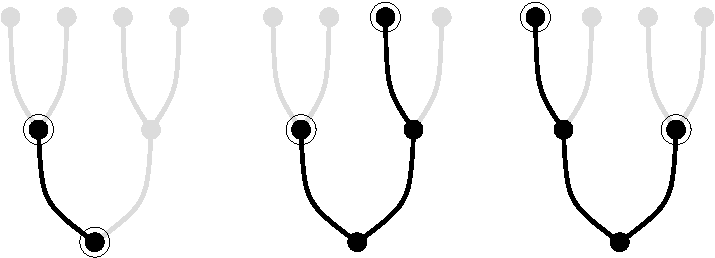
\includegraphics[scale=0.4]{figures/syntacMinim.pdf}\\
	  \begin{tikzpicture}[scale=1.5,font=\footnotesize]
			\tikzset{
				empty node/.style={circle,inner sep=0,fill=none},
				solid node/.style={circle,draw,inner sep=1.5,fill=black},
				hollow node/.style={circle,draw,inner sep=1.5,fill=white},
				gray node/.style={circle,draw={rgb:black,1;white,4},inner sep=1.5,fill={rgb:black,1;white,4}}
			}
			\tikzset{snake it/.style={decorate, decoration=snake, line cap=round}}
			\tikzset{gray line/.style={line cap=round,thick,color={rgb:black,1;white,4}}}
			\tikzset{thick line/.style={line cap=round,rounded corners=0.1mm,thick}}
			\node (a)[solid node] at (0,0) {};
			\node (a1)[gray node] at (0.3,0.5) {};
			\node (a0)[solid node] at (-0.3,0.5) {};
			\node (a00)[gray node] at (-0.45,1) {};
			\node (a01)[gray node] at (-0.15,1) {};
			\node (a10)[gray node] at (0.15,1) {};
			\node (a11)[gray node] at (0.45,1) {};
			\draw[-,thick line] (0,0) to (a0);
			\draw[-,gray line] (a) to (a1);
			\begin{pgfonlayer}{background}
			\draw[-,gray line] (a0) to (a00);
			\draw[-,gray line] (a0) to (a01);
			\end{pgfonlayer}
			\draw[-,gray line] (a1) to (a10);
			\draw[-,gray line] (a1) to (a11);
			\draw[fill=none] (a) circle [radius=0.75mm];
			\draw[fill=none] (a0) circle [radius=0.75mm];
		\end{tikzpicture}
		\hspace{5mm}
		\begin{tikzpicture}[scale=1.5,font=\footnotesize]
			\tikzset{
				empty node/.style={circle,inner sep=0,fill=none},
				solid node/.style={circle,draw,inner sep=1.5,fill=black},
				hollow node/.style={circle,draw,inner sep=1.5,fill=white},
				gray node/.style={circle,draw={rgb:black,1;white,4},inner sep=1.5,fill={rgb:black,1;white,4}}
			}
			\tikzset{snake it/.style={decorate, decoration=snake, line cap=round}}
			\tikzset{gray line/.style={line cap=round,thick,color={rgb:black,1;white,4}}}
			\tikzset{thick line/.style={line cap=round,rounded corners=0.1mm,thick}}
			\node (a)[solid node] at (0,0) {};
			\node (a1)[solid node] at (0.3,0.5) {};
			\node (a0)[solid node] at (-0.3,0.5) {};
			\node (a00)[gray node] at (-0.45,1) {};
			\node (a01)[gray node] at (-0.15,1) {};
			\node (a10)[solid node] at (0.15,1) {};
			\node (a11)[gray node] at (0.45,1) {};
			\draw[-,thick line] (0,0) to (a0);
			\draw[-,thick line] (a) to (a1);
			\begin{pgfonlayer}{background}
			\draw[-,gray line] (a0) to (a00);
			\draw[-,gray line] (a0) to (a01);
			\end{pgfonlayer}
			\draw[-,thick line] (a1) to (a10);
			\draw[-,gray line] (a1) to (a11);
			\draw[fill=none] (a0) circle [radius=0.75mm];
			\draw[fill=none] (a10) circle [radius=0.75mm];
		\end{tikzpicture}
		\hspace{5mm}
		\begin{tikzpicture}[scale=1.5,font=\footnotesize]
			\tikzset{
				empty node/.style={circle,inner sep=0,fill=none},
				solid node/.style={circle,draw,inner sep=1.5,fill=black},
				hollow node/.style={circle,draw,inner sep=1.5,fill=white},
				gray node/.style={circle,draw={rgb:black,1;white,4},inner sep=1.5,fill={rgb:black,1;white,4}}
			}
			\tikzset{snake it/.style={decorate, decoration=snake, line cap=round}}
			\tikzset{gray line/.style={line cap=round,thick,color={rgb:black,1;white,4}}}
			\tikzset{thick line/.style={line cap=round,rounded corners=0.1mm,thick}}
			\node (a)[solid node] at (0,0) {};
			\node (a1)[solid node] at (0.3,0.5) {};
			\node (a0)[solid node] at (-0.3,0.5) {};
			\node (a00)[solid node] at (-0.45,1) {};
			\node (a01)[gray node] at (-0.15,1) {};
			\node (a10)[gray node] at (0.15,1) {};
			\node (a11)[gray node] at (0.45,1) {};
			\draw[-,thick line] (0,0) to (a0);
			\draw[-,thick line] (a) to (a1);
			\begin{pgfonlayer}{background}
			\draw[-,thick line] (a0) to (a00);
			\draw[-,gray line] (a0) to (a01);
			\end{pgfonlayer}
			\draw[-,gray line] (a1) to (a10);
			\draw[-,gray line] (a1) to (a11);
			\draw[fill=none] (a00) circle [radius=0.75mm];
			\draw[fill=none] (a1) circle [radius=0.75mm];
		\end{tikzpicture}
	\end{center}\caption{An example of three tuple types on $[T]^{2}$, for a tree $T$ that syntactically minimizes the number of types.}\label{fig:lastminute1}
\end{figure}

We shall see that the number above is optimal. Of course, it is not the case that one of the above types can never be omitted in a perfect tree and it is in fact one difficulty in showing that a tree $T$ syntactically minimizing the number of tuple types really does so: every tuple type can be omitted in some perfect tree. Of course omitting a type may force some other type to become unavoidable. In order to overcome this difficulty, we need to introduce a third equivalence relation, within which we erase the part of a tuple type which can be omitted.

\begin{definition}\index{type!weak tuple}\index{weak tuple type}
The \emph{weak tuple types} are the equivalence classes of the following relation: $\overline{\sigma}, \overline{\tau}$ have the same weak tuple type if there is a bijection $f$ from $\overline{\sigma}^{cl}$ to $\overline{\tau}^{cl}$ such that:
\begin{itemize}
\item for $\sigma_1,\sigma_2 \in \overline{\sigma}^{cl}$ we have $\sigma_1 \preceq \sigma_2$ iff $f(\sigma_1) \preceq f(\sigma_2)$;
\item for $\sigma_1,\sigma_2,\sigma_3 \in \overline{\sigma}^{cl}$ we have $\sigma_1 0 \preceq \sigma_2$ and $\sigma_1 1 \preceq \sigma_3$ iff $f(\sigma_1) 0 \preceq f(\sigma_2)$ and $f(\sigma_1) 1 \preceq f(\sigma_3)$;
\item elements of $\overline{\sigma}$ are sent to $\overline{\tau}$.
\end{itemize}
\end{definition}

In other word, weak tuple types are tuple types, modulo the fact that whenever a node is not branching, it does not matter for its extension to go left or right. It is clear from the definition that the tuple types are a refinement of the weak tuple types. On the other hand neither the weak tuple types are a refinement of the embedding types, or the embedding types a refinement of the weak tuple types.

\begin{lemma} \label{lem:coincide_smntt}
Let $T$ be a perfect tree which syntactically minimizes the number of tuple types. Then its tuple types and weak tuple types coincide.
\end{lemma}
\begin{proof}
We already have that the tuple types are a refinement of the weak tuple types. All we have to do is to show that restricted to $T$, the weak tuple types are a refinement of the tuple types.

For any $n$ consider any two $n$-tuples $\overline{\sigma},\overline{\tau}$ of $T$. Suppose they are in the same weak tuple type via some bijection $f:\overline{\sigma}^{cl} \rightarrow \overline{\tau}^{cl}$. Let us show that $f$ in fact witnesses that $\overline{\sigma}$ and $\overline{\tau}$ are in the same tuple types. For that it is enough to show that $\sigma_1 i \preceq \sigma_2$ implies $f(\sigma_1) i \preceq f(\sigma_2)$ for $\sigma_1,\sigma_2 \in \overline{\sigma}^{cl}$. Let $\sigma_1,\sigma_2 \in \overline{\sigma}^{cl}$ with $\sigma_1 i \preceq \sigma_2$. 

Suppose first that we have a string $\sigma_3 \in \overline{\sigma}^{cl}$ such that $\sigma_1 (1-i) \preceq \sigma_3$. Then by definition of a weak tuple type we have $f(\sigma_1) i \preceq f(\sigma_2)$. Otherwise there are two possibilities: either $\sigma_1 \in \overline{\sigma}$ or $\sigma_1 \in \overline{\sigma}^{cl}$ but $\sigma_1 \notin \overline{\sigma}^{\wedge}$. 

In the first case, note that we must have a string $\sigma_3 \in \overline{\sigma}$ with $\sigma_1 i \preceq \sigma_2 \preceq \sigma_3$. Note that as $\sigma_1,\sigma_3 \in \overline{\sigma}$ then also $\sigma_1,\sigma_3 \in T$. Then by property (2) in \Cref{def:syntactic_minimize} (the definition of syntactically minimizing the number of tuple type), we have $\sigma_1 0 \preceq \sigma_2 \preceq \sigma_3$. Note also that $f(\sigma_1) \preceq f(\sigma_1) \preceq f(\sigma_3)$ and that by hypothesis on $f$ we have $f(\sigma_1),f(\sigma_3) \in \overline{\tau} \subseteq T$. Therefore also we have $f(\sigma_1)0 \prec f(\sigma_3)$ by (2) in \Cref{def:syntactic_minimize} and thus we have $f(\sigma_1)0 \prec f(\sigma_2)$.

In the second case we have $\sigma_1,\sigma_2 \in T^{cl}$ and $\sigma_1 \notin T^{\wedge}$. Thus by property (3) in \Cref{def:syntactic_minimize} we have $\sigma_1 0 \preceq \sigma_2$. We shall argue that also $f(\sigma_1) \notin T^{\wedge}$. Suppose for contradiction that $f(\sigma_1) \in T^{\wedge}$. Then also $f(\sigma_1) \in \overline{\tau}^{\wedge}$. Recall that by hypothesis $\sigma_1 \notin \overline{\sigma}$ and thus $f(\sigma_1) \notin \overline{\tau}$ (as $f$ is a bijection between the two). It follows that $f(\sigma_1)$ must be the meet of two nodes in $\overline{\tau}$ and thus is branching in $\overline{\tau}^{cl}$. On the other hand as $\sigma_1 \notin T^{\wedge}$ it is not branching in $\overline{\sigma}^{cl}$ which contradicts the properties of $f$. Thus $f(\sigma_1) \notin T^{\wedge}$ and it follows by property (3) in the definition of syntactically minimizes the number of tuple type that $f(\sigma_1) 0 \preceq f(\sigma_2)$.

We then have that $\overline{\sigma}$ and $\overline{\tau}$ are in the same tuple types.
\end{proof}

We shall now identify the weak tuple types no perfect tree can omit. We shall then see that weak tuple types of a tree which syntactically minimizes the number of tuple types are all of this form. It will then follow that such a tree really minimizes the number of tuple types.

\begin{definition}\index{tuple type!length-injective}
A tuple type (resp. a weak tuple type) $\overline{\sigma}$ is \emph{length-injective} if $\sigma_1,\sigma_2 \in \overline{\sigma}^{\wedge}$ implies $|\sigma_1| \neq |\sigma_2|$.
\end{definition}

\begin{definition}\index{tuple type!meet-avoiding}
A tuple type (resp. a weak tuple type) $\overline{\sigma}$ is \emph{meet-avoiding} if for any incomparable $\sigma_1,\sigma_2 \in \overline{\sigma}$ we have $\sigma_1 \wedge \sigma_2 \notin \overline{\sigma}$.
\end{definition}

See \Cref{fig:lastminute2} for an illustration. 
\begin{figure}
	\begin{center}
	  %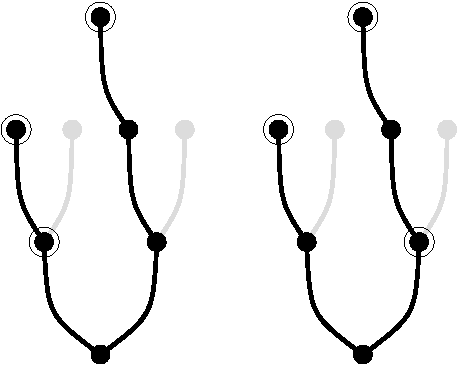
\includegraphics[scale=0.4]{figures/leninj-meetav.pdf}\\
	  \begin{tikzpicture}[scale=1.5,font=\footnotesize]
			\tikzset{
				empty node/.style={circle,inner sep=0,fill=none},
				solid node/.style={circle,draw,inner sep=1.5,fill=black},
				hollow node/.style={circle,draw,inner sep=1.5,fill=white},
				gray node/.style={circle,draw={rgb:black,1;white,4},inner sep=1.5,fill={rgb:black,1;white,4}}
			}
			\tikzset{snake it/.style={decorate, decoration=snake, line cap=round}}
			\tikzset{gray line/.style={line cap=round,thick,color={rgb:black,1;white,4}}}
			\tikzset{thick line/.style={line cap=round,rounded corners=0.1mm,thick}}
			\node (a)[solid node] at (0,0) {};
			\node (a1)[solid node] at (0.3,0.5) {};
			\node (a0)[solid node] at (-0.3,0.5) {};
			\node (a00)[solid node] at (-0.45,1) {};
			\node (a01)[gray node] at (-0.15,1) {};
			\node (a10)[solid node] at (0.15,1) {};
			\node (a11)[gray node] at (0.45,1) {};
			\node (a100)[solid node] at (0.1,1.5) {};
			\draw[-,thick line] (a) to (a0);
			\draw[-,thick line] (a) to (a1);
			\begin{pgfonlayer}{background}
			\draw[-,thick line] (a0) to (a00);
			\draw[-,gray line] (a0) to (a01);
			\end{pgfonlayer}
			\draw[-,thick line] (a1) to (a10);
			\draw[-,thick line] (a10) to (a100);
			\draw[-,gray line] (a1) to (a11);
			\draw[fill=none] (a0) circle [radius=0.75mm];
			\draw[fill=none] (a00) circle [radius=0.75mm];
			\draw[fill=none] (a100) circle [radius=0.75mm];
		\end{tikzpicture}
		\hspace{5mm}
		\begin{tikzpicture}[scale=1.5,font=\footnotesize]
			\tikzset{
				empty node/.style={circle,inner sep=0,fill=none},
				solid node/.style={circle,draw,inner sep=1.5,fill=black},
				hollow node/.style={circle,draw,inner sep=1.5,fill=white},
				gray node/.style={circle,draw={rgb:black,1;white,4},inner sep=1.5,fill={rgb:black,1;white,4}}
			}
			\tikzset{snake it/.style={decorate, decoration=snake, line cap=round}}
			\tikzset{gray line/.style={line cap=round,thick,color={rgb:black,1;white,4}}}
			\tikzset{thick line/.style={line cap=round,rounded corners=0.1mm,thick}}
			\node (a)[solid node] at (0,0) {};
			\node (a1)[solid node] at (0.3,0.5) {};
			\node (a0)[solid node] at (-0.3,0.5) {};
			\node (a00)[solid node] at (-0.45,1) {};
			\node (a01)[gray node] at (-0.15,1) {};
			\node (a10)[solid node] at (0.15,1) {};
			\node (a11)[gray node] at (0.45,1) {};
			\node (a100)[solid node] at (0.1,1.5) {};
			\draw[-,thick line] (a) to (a0);
			\draw[-,thick line] (a) to (a1);
			\begin{pgfonlayer}{background}
			\draw[-,thick line] (a0) to (a00);
			\draw[-,gray line] (a0) to (a01);
			\end{pgfonlayer}
			\draw[-,thick line] (a1) to (a10);
			\draw[-,thick line] (a10) to (a100);
			\draw[-,gray line] (a1) to (a11);
			\draw[fill=none] (a1) circle [radius=0.75mm];
			\draw[fill=none] (a00) circle [radius=0.75mm];
			\draw[fill=none] (a100) circle [radius=0.75mm];
		\end{tikzpicture}
	\end{center}\caption{An example of two length-injective and meet-avoiding tuple types, generating the same embedding type.}\label{fig:lastminute2}
\end{figure}
%\todo[inline]{Paul-Elliot, can you please put the example: $0, 00, 100$ and $1, 00, 100$}

Up to symmetry and restricted to a tree which syntactically minimizes the number of types, these are the only tuple types generated by three strings and which are in the same embedding type. We will now see that the length-injective and meet-avoiding weak tuple types are exactly those which cannot be avoided by a perfect tree.

\begin{lemma} \label{lem:doesnotavoid_smntt}
Let $S$ be any perfect tree. Then $S$ has a member inside every length-injective and meet-avoiding weak tuple type.
\end{lemma}
\begin{proof}
Let $\overline{\sigma}$ be a length-injective and meet-avoiding tuple type. Let us define first an injection $f$ from $\overline{\sigma}^{\wedge}$ into $S^{\wedge}$ with the following properties:
\begin{enumerate}
\item[(1)] $f(\overline{\sigma}) \subseteq S$;
\item[(2)] for $\sigma_1,\sigma_2 \in \overline{\sigma}^{\wedge}$ we have $\sigma_1 \preceq \sigma_2$ iff $f(\sigma_1) \preceq f(\sigma_2)$;
\item[(3)] if $\sigma_1$ is branching in $\overline{\sigma}^{\wedge}$ then $f(\sigma_1)$ is branching in $S^\wedge$. Furthermore for $\sigma_1,\sigma_2, \sigma_3 \in \overline{\sigma}^{\wedge}$ we have $\sigma_1 0 \preceq \sigma_2$ and $\sigma_1 1 \preceq \sigma_3$ iff $f(\sigma_1) 0 \preceq f(\sigma_2)$ and $f(\sigma_1) 1 \preceq f(\sigma_3)$;
\item[(4)] for $\sigma_1,\sigma_2 \in \overline{\sigma}^{\wedge}$ we have $|\sigma_1| < |\sigma_2|$ iff $|f(\sigma_1)| < |f(\sigma_2)|$.
\end{enumerate}

Let $\sigma_1, \dots, \sigma_n$ be a list of the elements of $\overline{\sigma}^{\wedge}$ with $|\sigma_1| < |\sigma_2| < \dots < |\sigma_n|$. Note that we must have $\sigma_i \preceq \sigma_j$ implies $i \leq j$. Note also that as $\overline{\sigma}$ is meet-avoiding we must have that $\rho \in \overline{\sigma}^\wedge$ is branching in $\overline{\sigma}^\wedge$ iff $\rho \notin \overline{\sigma}$.


If $\sigma_1 \in \overline{\sigma}$ then find the lexicographically first $\tau \in S$ and let $f(\sigma_1) = \tau$. Otherwise find the lexicographically first $\tau \in S^\wedge$ which is branching in $S^\wedge$ and let $f(\sigma_1) = \tau$. Note that so far (1)(2)(3) and (4) are satisfied.

Suppose $f(\sigma_1), \dots, f(\sigma_k)$ have been defined with (1)(2)(3) and (4) satisfied so far. Consider $\sigma_{k+1}$. Let $j \leq k$ be the largest such that $\sigma_{j} \prec \sigma_{k+1}$. Suppose first $\sigma_j$ is branching in $\overline{\sigma}^{\wedge}$. Then by induction hypothesis (3) we must have that $f(\sigma_j)$ is branching in $S^{\wedge}$. In this case let $i \in \{0,1\}$ be such that $\sigma_{j} i \preceq \sigma_{k+1}$. If $\sigma_{k+1} \in \overline{\sigma}$ then find the lexicographically first $\tau \in S$ such that $|\tau| > |f(\sigma_k)|$ and such that $f(\sigma_j) i \preceq \tau$. Then let $f(\sigma_{k+1}) = \tau$. Otherwise find the lexicographically first branching $\tau \in S^{\wedge}$, such that $|\tau| > |f(\sigma_k)|$ and such that $f(\sigma_j) i \preceq \tau$. Then let $f(\sigma_{k+1}) = \tau$. Note that in any case (1) (2) (3) and (4) are satisfied so far.

Suppose now $\sigma_j$ is not branching in $\overline{\sigma}^{\wedge}$. If $\sigma_{k+1} \in \overline{\sigma}$ then find the lexicographically first $\tau \in S$ such that $|\tau| > |f(\sigma_k)|$ and such that $f(\sigma_j) \preceq \tau$. Then let $f(\sigma_{k+1}) = \tau$. Otherwise find the lexicographically first branching $\tau \in S^{\wedge}$, such that $|\tau| > |f(\sigma_k)|$ and such that $f(\sigma_j) \preceq \tau$. Then let $f(\sigma_{k+1}) = \tau$. Note that in any case (1) (2) (3) and (4) are satisfied so far. This ends the first part of the construction.

Note also that $f$ is a bijection between $\overline{\sigma}$ and $f(\overline{\sigma}) \subseteq S$. In order to show that $\overline{\sigma}$ and $f(\overline{\sigma})$ are in the same weak tuple type, we shall now extend $f$ to $\overline{\sigma}^{cl}$ such that $f$ becomes a bijection from $\overline{\sigma}^{cl}$ to $f(\overline{\sigma})^{cl}$.

Let us first argue that so far $f$ is a bijection from $\overline{\sigma}^{\wedge}$ to $f(\overline{\sigma})^{\wedge}$. We have $f(\overline{\sigma}) \subseteq f(\overline{\sigma}^{\wedge})$. By design we also have that $f(\overline{\sigma}^{\wedge})$ is meet closed and thus we have $f(\overline{\sigma})^{\wedge} = f(\overline{\sigma}^{\wedge})$. As $f$ is injective it is a bijection from $\overline{\sigma}^{\wedge}$ to $f(\overline{\sigma}^\wedge)$ and then it is a bijection from $\overline{\sigma}^{\wedge}$ to $f(\overline{\sigma})^\wedge$.

Let us now extend $f$ to $\overline{\sigma}^{cl}$: for incomparable $\sigma_1,\sigma_2 \in \overline{\sigma}^{\wedge}$ with $|\sigma_1| < |\sigma_2|$ we assign $f(\sigma_2 \upharpoonright {|\sigma_1|})$ to $f(\sigma_2)  \upharpoonright {|f(\sigma_1)|}$. Let us now show that $f(\overline{\sigma}^{cl}) = f(\overline{\sigma})^{cl}$. It is clear by definition of $f$ that $f(\overline{\sigma}^{cl}) \subseteq f(\overline{\sigma})^{cl}$. Let us now show $f(\overline{\sigma})^{cl} \subseteq f(\overline{\sigma}^{cl})$.

Suppose $\tau \in f(\overline{\sigma})^{cl}$. Then as $f(\overline{\sigma})^{cl} = (f(\overline{\sigma})^{\wedge})^{cl} = f(\overline{\sigma}^{\wedge})^{cl}$ we have $\tau \in f(\overline{\sigma}^{\wedge})^{cl}$. Then there exists $\sigma_1,\sigma_2 \in \overline{\sigma}^{\wedge}$ with $|f(\sigma_1)| < |f(\sigma_2)|$ and with $\tau = f(\sigma_2) \upharpoonright {|f(\sigma_1)|}$. By (4) we have $|\sigma_1| < |\sigma_2|$ and then $\sigma_2 \upharpoonright {|\sigma_1|} \in \overline{\sigma}^{cl}$. Thus $\tau \in f(\overline{\sigma}^{cl})$ and then $f(\overline{\sigma})^{cl} \subseteq f(\overline{\sigma}^{cl})$ and then $f(\overline{\sigma})^{cl} = f(\overline{\sigma}^{cl})$.

Let us now show that $f$ is injective on $\overline{\sigma}^{cl}$. Let $\sigma_1,\sigma_2, \rho_1, \rho_2 \in \overline{\sigma}^{\wedge}$ with $\sigma_1,\sigma_2$ and $\rho_1,\rho_2$ incomparable, with $|\sigma_1| < |\sigma_2|$ and with $|\rho_1| < |\rho_2|$. Suppose $\sigma_2 \upharpoonright {|\sigma_1|} \neq \rho_2 \upharpoonright {|\rho_1|}$. If $\sigma_1 \neq \rho_1$ then by (4) we must have $|f(\sigma_1)| \neq |f(\rho_1)|$ and thus $f(\sigma_2)  \upharpoonright {|f(\sigma_1)|} \neq f(\rho_2)  \upharpoonright {|f(\rho_1)|}$. Otherwise it must be that $\sigma_2 \upharpoonright {s} \neq \rho_2 \upharpoonright {s}$ for $s = |\sigma_1| = |\rho_1|$. By definition of $f$ it must be that $f((\sigma_2 \upharpoonright {s}) \wedge (\rho_2 \upharpoonright {s})) = f(\sigma_2 \upharpoonright {s}) \wedge f(\rho_2 \upharpoonright {s})$ and thus by (3) that $f(\sigma_2 \upharpoonright {s}) \neq f(\rho_2 \upharpoonright {s})$. 

It follows that $f$ is a bijection from $\overline{\sigma}^{cl}$ to $f(\overline{\sigma}^{cl})$ and thus that it is a bijection from $\overline{\sigma}^{cl}$ to $f(\overline{\sigma})^{cl}$.

It is clear that property (1) and (2) is still satisfied by $f$ on $\overline{\sigma}^{cl}$. Also as every branching node of $\overline{\sigma}^{cl}$ is already branching in $\overline{\sigma}^{\wedge}$ property (3) is till satisfied on $\overline{\sigma}^{cl}$. It follows that $\overline{\sigma}$ and $f(\overline{\sigma})$ are in the same weak tuple type.
\end{proof}

\begin{lemma} \label{lem:realizeall_smntt}
Let $T$ be a tree which syntactically minimizes the number of tuple types. Then every weak tuple type of $T$ is length-injective and meet-avoiding.
\end{lemma}
\begin{proof}
By definition we have that $\sigma_1,\sigma_2 \in T^{\wedge}$ implies $|\sigma_1| \neq |\sigma_2|$. Thus the weak tuple types of $T$ are length-injective. Suppose now $\sigma_1,\sigma_2 \in T$ with $\sigma_1,\sigma_2$ incomparable. Suppose for contradiction that $\sigma_1 \wedge \sigma_2 \in T$. Then we have $(\sigma_1 \wedge \sigma_2) 1 \preceq \sigma_1$ or $(\sigma_1 \wedge \sigma_2) 1 \preceq \sigma_2$. In any case we violate property (2) of syntactically minimizing the number of types. Thus for any $\sigma_1,\sigma_2 \in T$ with $\sigma_1,\sigma_2$ incomparable we have $\sigma_1 \wedge \sigma_2 \notin T$ which implies that the weak tuple types of $T$ are meet-avoiding.
\end{proof}

\section{Generalized CHM tree theorem}

We are now ready to study the generalized CHM tree theorem, where we do not necessarily required the subtree to be a strong subtree.

\begin{definition}\index{$t^T_{\TT}(n)$}
Given a perfect tree $T$, let $t^T_{\TT}(n)$ be the number of tuple types generated by $n$ distinct strings of $T$. Let 
$$t_{\TT}(n) = \min \{t^T_{\TT}(n)\:\ T \text{ is a perfect tree}\}.$$
\end{definition}

\begin{theorem} \label{th:reallyminimizes}
Suppose $T$ syntactically minimizes the number of tuple types, then $t_{\TT}(n) = t_{\TT}^T(n)$.
\end{theorem}
\begin{proof}
Suppose $T$ syntactically minimizes the number of tuple types. Then by \Cref{lem:coincide_smntt} the tuple types of $T$ coincide with its weak tuple types. By \Cref{lem:realizeall_smntt} every weak tuple type of $T$ is length-injective and meet-avoiding. By \Cref{lem:doesnotavoid_smntt} we then have that every weak-tuple type of $T$ is a weak-tuple type in any perfect tree $S$. Using the fact that the tuple types are a refinement of the weak tuple types, we then have that given any $n$, the number of tuple types of $[S]^{n}$ is bigger than the number of weak tuple types of $[S]^{n}$ and then bigger than the number of weak tuple types of $[T]^{n}$ and then bigger than the number of tuple types of $[T]^{n}$. Thus $t_{\TT}(n) = t_{\TT}^T(n)$.
\end{proof}

\begin{theorem}[Generalized CHM tree theorem]
For every $n$, the principle $\mathrm{CMHTT^n_{k,t_{\TT}(n)}}$ is provable in $\ACA_0$ but $\RCA_0$ proves that the principle $\mathrm{CMHTT^n_{k,t_{\TT}(n)-1}}$ is false.
\end{theorem}
\begin{proof}
Let $\Mc$ be a model of $\ACA_0$. Let $T \in \Mc$ be a perfect tree and $c \in \Mc$ be a color of $[T]^n$. Using \Cref{th:strong_gen_treeth}, there is a strong subtree $S \subseteq T$ such that every tuple type of $[S]^n$ is monochromatic for $c$. Using \Cref{lem:existance_smntt} let $R$ be a $S$-computable perfect subtree of $S$ which synctactically minimizes the number of tuple types. Note that $R \in \Mc$ and that by \Cref{th:reallyminimizes} $[R]^n$ has at most $t_{\TT}(n)$ many tuple types. It follows that $c$ uses at most $t_{\TT}(n)$ many colors on $R$.

To show optimality, and given an enumeration $\{\embfont e_i\}_{i \leq t_{\sTT}(n)}$ of the tuple types generated by $n$ strings, let us define a color on $2^{<\omega}$ which associates $i$ to $\overline{\sigma}$ of tuple type $\embfont e_i$. By minimality of $t_{\TT}(n)$ among $t^T_{\TT}(n)$ for a perfect tree $T$ we have that every perfect subtree of $2^{<\omega}$ uses at least $t_{\TT}(n)$ colors.
\end{proof}

\begin{theorem}[CHM tree theorem for $n$-tuple and $k$-colors]
For every coloring of $n$-tuples of pairwise comparable strings, there exists a perfect tree on which the coloring is monochromatic.
\end{theorem}
\begin{proof}
This follows from the fact that given any $n$, there is only one weak tuple type of size $n$ which contains only comparable strings.
\end{proof}

It is easy to determine the number $e_n$ of embedding types of height $n$, which is given by the following induction:

$$
\begin{array}{rcl}
e_0&=&1,\\
e_1&=&1,\\
e_{n+1}&=&2 \times e_n \times (\sum_{i<n} e_i) + e_n^2.
\end{array}
$$
%
The definition above is justified by the following observation: there is one tree of height $0$ (the emptyset), there is one tree of height $1$ (the empty string) and for any $n \geq 1$, the possibilities to build trees of height $n+1$ are as follow: having a left subtree of the root (the empty string) of height $n$ and a right subtree of the root of height $<n$, or the inverse of that, or have both a left and a right subtree of the root of height $n$. 

The number of embedding types generated by $n$ strings, namely $e_{\sTT}(n)$ appears much harder to compute. It is the same for $t_{\sTT}(n)$ and $t_{\TT}(n)$. We can also define the function $n \mapsto e_{\TT}(n)$ which to $n$ associates the minimal number of embedding type within any perfect tree (which is the number of embedding types generated by $n$ strings of a tree which syntactically minimizes the number of tuple types).

We computed the first values of each with the help of a computer program:

$$
\begin{array}{|c|c|c|c|c|}
\hline
&e_{\sTT}&t_{\sTT}&e_{\TT}&t_{\TT}\\
\hline
\hline
0&1&1&1&1\\
\hline
1&1&1&1&1\\
\hline
2&7&7&3&3\\
\hline
3&345&369&27&29\\
\hline
4&136949&145215&561&635\\
\hline
\end{array}
$$

None of these sequence appears in OEIS, The On-Line Encyclopedia of Integer Sequences \cite{OEIS}. It then seems that each of them is a new natural combinatorial sequence. Even if it seems that these sequences cannot be computed with an easy mathematical induction like for the number of embedding types of height $n$, we conjecture each of them to be polynomial time computable.

%%% Local Variables:
%%% mode: latex
%%% TeX-master: "../embryon"
%%% End:
